\documentclass[12pt,a4paper]{article}
        \usepackage{graphicx}
        \usepackage{geometry}
        \geometry{margin=2cm}
        \usepackage{helvet}
        \usepackage{xcolor}
        \usepackage{amsmath} % for bmatrix
        \setlength{\parindent}{0pt}  % No indentation globally
        \renewcommand{\familydefault}{\sfdefault}
        \usepackage[german]{babel}% for glqq / grqq

        \begin{document}\begin{center}
                \Huge \textbf{Hexafluorobenzene} \\[1cm]
                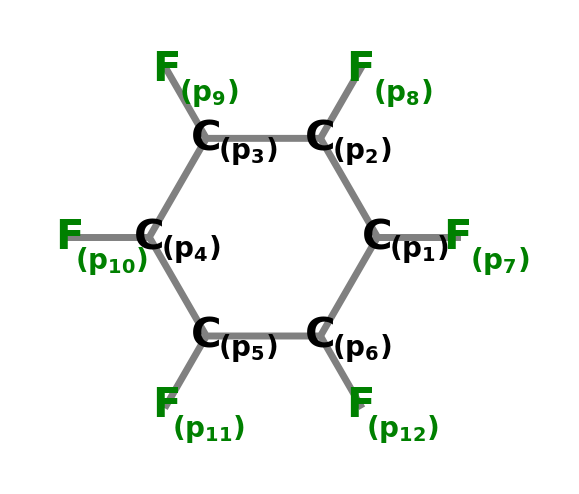
\includegraphics[width=0.5\textwidth]{hexafluorobenzene} \\[0.5cm]
                \Large Point Group: \textbf{D6h}
            \end{center}\newpage\section*{p orbitals}
Symmetry behavior of the p-orbitals:
$$\mathsf{\Gamma}_{red} = \,12 E\;; \,-4 C'2\;; \,-12 \sigma h\;; \,4 \sigma v\;$$
$$\mathsf{\Gamma}_{irred} = \,2 B2g\;\oplus{}\,2 E1g\;\oplus{}\,2 A2u\;\oplus{}\,2 E2u\;$$


\begin{itemize}
\item SALC of B2g: \quad $\frac{\sqrt{6} \left(\text{p}_{1} - \text{p}_{2} + \text{p}_{3} - \text{p}_{4} + \text{p}_{5} - \text{p}_{6}\right)}{6}$
\item SALC of B2g: \quad $\frac{\sqrt{6} \left(- \text{p}_{10} + \text{p}_{11} - \text{p}_{12} + \text{p}_{7} - \text{p}_{8} + \text{p}_{9}\right)}{6}$
\item SALC of E1g: \quad $\frac{\sqrt{3} \left(2 \text{p}_{1} + \text{p}_{2} - \text{p}_{3} - 2 \text{p}_{4} - \text{p}_{5} + \text{p}_{6}\right)}{6}$
\item SALC of E1g: \quad $\frac{\sqrt{3} \left(\text{p}_{1} + 2 \text{p}_{2} + \text{p}_{3} - \text{p}_{4} - 2 \text{p}_{5} - \text{p}_{6}\right)}{6}$
\item SALC of E1g: \quad $\frac{\sqrt{3} \left(- \text{p}_{1} + \text{p}_{2} + 2 \text{p}_{3} + \text{p}_{4} - \text{p}_{5} - 2 \text{p}_{6}\right)}{6}$
\item SALC of E1g: \quad $\frac{\sqrt{3} \left(- \text{p}_{10} - 2 \text{p}_{11} - \text{p}_{12} + \text{p}_{7} + 2 \text{p}_{8} + \text{p}_{9}\right)}{6}$
\item SALC of A2u: \quad $\frac{\sqrt{6} \left(\text{p}_{1} + \text{p}_{2} + \text{p}_{3} + \text{p}_{4} + \text{p}_{5} + \text{p}_{6}\right)}{6}$
\item SALC of A2u: \quad $\frac{\sqrt{6} \left(\text{p}_{10} + \text{p}_{11} + \text{p}_{12} + \text{p}_{7} + \text{p}_{8} + \text{p}_{9}\right)}{6}$
\item SALC of E2u: \quad $\frac{\sqrt{3} \left(2 \text{p}_{1} - \text{p}_{2} - \text{p}_{3} + 2 \text{p}_{4} - \text{p}_{5} - \text{p}_{6}\right)}{6}$
\item SALC of E2u: \quad $\frac{\sqrt{3} \left(- \text{p}_{1} + 2 \text{p}_{2} - \text{p}_{3} - \text{p}_{4} + 2 \text{p}_{5} - \text{p}_{6}\right)}{6}$
\item SALC of E2u: \quad $\frac{\sqrt{3} \left(- \text{p}_{1} - \text{p}_{2} + 2 \text{p}_{3} - \text{p}_{4} - \text{p}_{5} + 2 \text{p}_{6}\right)}{6}$
\item SALC of E2u: \quad $\frac{\sqrt{3} \left(\text{p}_{10} + \text{p}_{11} - 2 \text{p}_{12} + \text{p}_{7} + \text{p}_{8} - 2 \text{p}_{9}\right)}{6}$
\end{itemize}
Put together these SALCs form the following Hamilton matrices:
     $$ H_{B2g}= \begin{pmatrix}\tilde{\alpha} - 2 \tilde{\beta} & 0\\0 & \tilde{\alpha}_{F}\end{pmatrix}$$ 
     $$ H_{E1g}= \begin{pmatrix}\tilde{\alpha} + \tilde{\beta} & \frac{\tilde{\alpha}}{2} + \frac{\tilde{\beta}}{2} & - \frac{\tilde{\alpha}}{2} - \frac{\tilde{\beta}}{2} & 0\\\frac{\tilde{\alpha}}{2} + \frac{\tilde{\beta}}{2} & \tilde{\alpha} + \tilde{\beta} & \frac{\tilde{\alpha}}{2} + \frac{\tilde{\beta}}{2} & 0\\- \frac{\tilde{\alpha}}{2} - \frac{\tilde{\beta}}{2} & \frac{\tilde{\alpha}}{2} + \frac{\tilde{\beta}}{2} & \tilde{\alpha} + \tilde{\beta} & 0\\0 & 0 & 0 & \tilde{\alpha}_{F}\end{pmatrix}$$ 
     $$ H_{A2u}= \begin{pmatrix}\tilde{\alpha} + 2 \tilde{\beta} & 6 \tilde{\beta}_{F}\\6 \tilde{\beta}_{F} & \tilde{\alpha}_{F}\end{pmatrix}$$ 
     $$ H_{E2u}= \begin{pmatrix}\tilde{\alpha} - \tilde{\beta} & - \frac{\tilde{\alpha}}{2} + \frac{\tilde{\beta}}{2} & - \frac{\tilde{\alpha}}{2} + \frac{\tilde{\beta}}{2} & 0\\- \frac{\tilde{\alpha}}{2} + \frac{\tilde{\beta}}{2} & \tilde{\alpha} - \tilde{\beta} & - \frac{\tilde{\alpha}}{2} + \frac{\tilde{\beta}}{2} & 0\\- \frac{\tilde{\alpha}}{2} + \frac{\tilde{\beta}}{2} & - \frac{\tilde{\alpha}}{2} + \frac{\tilde{\beta}}{2} & \tilde{\alpha} - \tilde{\beta} & 0\\0 & 0 & 0 & \tilde{\alpha}_{F}\end{pmatrix}$$ 


Solving Hückels secular equations, that follow from these H, leads to:
\begin{itemize}
\item orbital of A2u with energy = 
                                $\frac{\tilde{\alpha}}{2} + \frac{\tilde{\alpha}_{F}}{2} + \tilde{\beta} - \frac{\sqrt{\tilde{\alpha}^{2} - 2 \tilde{\alpha} \tilde{\alpha}_{F} + 4 \tilde{\alpha} \tilde{\beta} + \tilde{\alpha}_{F}^{2} - 4 \tilde{\alpha}_{F} \tilde{\beta} + 4 \tilde{\beta}^{2} + 144 \tilde{\beta}_{F}^{2}}}{2}$ \\
( 
$$
\begin{pmatrix}- \frac{12 \tilde{\beta}_{F}}{\sqrt{144 \left|{\frac{\tilde{\beta}_{F}}{\tilde{\alpha} - \tilde{\alpha}_{F} + 2 \tilde{\beta} + \sqrt{\tilde{\alpha}^{2} - 2 \tilde{\alpha} \tilde{\alpha}_{F} + 4 \tilde{\alpha} \tilde{\beta} + \tilde{\alpha}_{F}^{2} - 4 \tilde{\alpha}_{F} \tilde{\beta} + 4 \tilde{\beta}^{2} + 144 \tilde{\beta}_{F}^{2}}}}\right|^{2} + 1} \left(\tilde{\alpha} - \tilde{\alpha}_{F} + 2 \tilde{\beta} + \sqrt{\tilde{\alpha}^{2} - 2 \tilde{\alpha} \tilde{\alpha}_{F} + 4 \tilde{\alpha} \tilde{\beta} + \tilde{\alpha}_{F}^{2} - 4 \tilde{\alpha}_{F} \tilde{\beta} + 4 \tilde{\beta}^{2} + 144 \tilde{\beta}_{F}^{2}}\right)} & \frac{1}{\sqrt{144 \left|{\frac{\tilde{\beta}_{F}}{\tilde{\alpha} - \tilde{\alpha}_{F} + 2 \tilde{\beta} + \sqrt{\tilde{\alpha}^{2} - 2 \tilde{\alpha} \tilde{\alpha}_{F} + 4 \tilde{\alpha} \tilde{\beta} + \tilde{\alpha}_{F}^{2} - 4 \tilde{\alpha}_{F} \tilde{\beta} + 4 \tilde{\beta}^{2} + 144 \tilde{\beta}_{F}^{2}}}}\right|^{2} + 1}}\end{pmatrix} * \left(\begin{array}{c}\text{1. SALC in A2u} \\ \text{2. SALC in A2u}\end{array}\right) = \begin{pmatrix}- \frac{12 \tilde{\beta}_{F}}{\sqrt{144 \left|{\frac{\tilde{\beta}_{F}}{\tilde{\alpha} - \tilde{\alpha}_{F} + 2 \tilde{\beta} + \sqrt{\tilde{\alpha}^{2} - 2 \tilde{\alpha} \tilde{\alpha}_{F} + 4 \tilde{\alpha} \tilde{\beta} + \tilde{\alpha}_{F}^{2} - 4 \tilde{\alpha}_{F} \tilde{\beta} + 4 \tilde{\beta}^{2} + 144 \tilde{\beta}_{F}^{2}}}}\right|^{2} + 1} \left(\tilde{\alpha} - \tilde{\alpha}_{F} + 2 \tilde{\beta} + \sqrt{\tilde{\alpha}^{2} - 2 \tilde{\alpha} \tilde{\alpha}_{F} + 4 \tilde{\alpha} \tilde{\beta} + \tilde{\alpha}_{F}^{2} - 4 \tilde{\alpha}_{F} \tilde{\beta} + 4 \tilde{\beta}^{2} + 144 \tilde{\beta}_{F}^{2}}\right)} & \frac{1}{\sqrt{144 \left|{\frac{\tilde{\beta}_{F}}{\tilde{\alpha} - \tilde{\alpha}_{F} + 2 \tilde{\beta} + \sqrt{\tilde{\alpha}^{2} - 2 \tilde{\alpha} \tilde{\alpha}_{F} + 4 \tilde{\alpha} \tilde{\beta} + \tilde{\alpha}_{F}^{2} - 4 \tilde{\alpha}_{F} \tilde{\beta} + 4 \tilde{\beta}^{2} + 144 \tilde{\beta}_{F}^{2}}}}\right|^{2} + 1}}\end{pmatrix} * \begin{pmatrix}\frac{\sqrt{6} \text{p}_{1}}{6} + \frac{\sqrt{6} \text{p}_{2}}{6} + \frac{\sqrt{6} \text{p}_{3}}{6} + \frac{\sqrt{6} \text{p}_{4}}{6} + \frac{\sqrt{6} \text{p}_{5}}{6} + \frac{\sqrt{6} \text{p}_{6}}{6}\\\frac{\sqrt{6} \text{p}_{10}}{6} + \frac{\sqrt{6} \text{p}_{11}}{6} + \frac{\sqrt{6} \text{p}_{12}}{6} + \frac{\sqrt{6} \text{p}_{7}}{6} + \frac{\sqrt{6} \text{p}_{8}}{6} + \frac{\sqrt{6} \text{p}_{9}}{6}\end{pmatrix} 
 $$ $$ = \frac{\sqrt{6} \left(- 12 \tilde{\beta}_{F} \left(\text{p}_{1} + \text{p}_{2} + \text{p}_{3} + \text{p}_{4} + \text{p}_{5} + \text{p}_{6}\right) + \left(\tilde{\alpha} - \tilde{\alpha}_{F} + 2 \tilde{\beta} + \sqrt{\tilde{\alpha}^{2} - 2 \tilde{\alpha} \tilde{\alpha}_{F} + 4 \tilde{\alpha} \tilde{\beta} + \tilde{\alpha}_{F}^{2} - 4 \tilde{\alpha}_{F} \tilde{\beta} + 4 \tilde{\beta}^{2} + 144 \tilde{\beta}_{F}^{2}}\right) \left(\text{p}_{10} + \text{p}_{11} + \text{p}_{12} + \text{p}_{7} + \text{p}_{8} + \text{p}_{9}\right)\right)}{6 \sqrt{144 \left|{\frac{\tilde{\beta}_{F}}{\tilde{\alpha} - \tilde{\alpha}_{F} + 2 \tilde{\beta} + \sqrt{\tilde{\alpha}^{2} - 2 \tilde{\alpha} \tilde{\alpha}_{F} + 4 \tilde{\alpha} \tilde{\beta} + \tilde{\alpha}_{F}^{2} - 4 \tilde{\alpha}_{F} \tilde{\beta} + 4 \tilde{\beta}^{2} + 144 \tilde{\beta}_{F}^{2}}}}\right|^{2} + 1} \left(\tilde{\alpha} - \tilde{\alpha}_{F} + 2 \tilde{\beta} + \sqrt{\tilde{\alpha}^{2} - 2 \tilde{\alpha} \tilde{\alpha}_{F} + 4 \tilde{\alpha} \tilde{\beta} + \tilde{\alpha}_{F}^{2} - 4 \tilde{\alpha}_{F} \tilde{\beta} + 4 \tilde{\beta}^{2} + 144 \tilde{\beta}_{F}^{2}}\right)} 
 $$ 
 )

\item orbital of A2u with energy = 
                                $\frac{\tilde{\alpha}}{2} + \frac{\tilde{\alpha}_{F}}{2} + \tilde{\beta} + \frac{\sqrt{\tilde{\alpha}^{2} - 2 \tilde{\alpha} \tilde{\alpha}_{F} + 4 \tilde{\alpha} \tilde{\beta} + \tilde{\alpha}_{F}^{2} - 4 \tilde{\alpha}_{F} \tilde{\beta} + 4 \tilde{\beta}^{2} + 144 \tilde{\beta}_{F}^{2}}}{2}$ \\
( 
$$
\begin{pmatrix}- \frac{12 \tilde{\beta}_{F}}{\sqrt{144 \left|{\frac{\tilde{\beta}_{F}}{\tilde{\alpha} - \tilde{\alpha}_{F} + 2 \tilde{\beta} - \sqrt{\tilde{\alpha}^{2} - 2 \tilde{\alpha} \tilde{\alpha}_{F} + 4 \tilde{\alpha} \tilde{\beta} + \tilde{\alpha}_{F}^{2} - 4 \tilde{\alpha}_{F} \tilde{\beta} + 4 \tilde{\beta}^{2} + 144 \tilde{\beta}_{F}^{2}}}}\right|^{2} + 1} \left(\tilde{\alpha} - \tilde{\alpha}_{F} + 2 \tilde{\beta} - \sqrt{\tilde{\alpha}^{2} - 2 \tilde{\alpha} \tilde{\alpha}_{F} + 4 \tilde{\alpha} \tilde{\beta} + \tilde{\alpha}_{F}^{2} - 4 \tilde{\alpha}_{F} \tilde{\beta} + 4 \tilde{\beta}^{2} + 144 \tilde{\beta}_{F}^{2}}\right)} & \frac{1}{\sqrt{144 \left|{\frac{\tilde{\beta}_{F}}{\tilde{\alpha} - \tilde{\alpha}_{F} + 2 \tilde{\beta} - \sqrt{\tilde{\alpha}^{2} - 2 \tilde{\alpha} \tilde{\alpha}_{F} + 4 \tilde{\alpha} \tilde{\beta} + \tilde{\alpha}_{F}^{2} - 4 \tilde{\alpha}_{F} \tilde{\beta} + 4 \tilde{\beta}^{2} + 144 \tilde{\beta}_{F}^{2}}}}\right|^{2} + 1}}\end{pmatrix} * \left(\begin{array}{c}\text{1. SALC in A2u} \\ \text{2. SALC in A2u}\end{array}\right) = \begin{pmatrix}- \frac{12 \tilde{\beta}_{F}}{\sqrt{144 \left|{\frac{\tilde{\beta}_{F}}{\tilde{\alpha} - \tilde{\alpha}_{F} + 2 \tilde{\beta} - \sqrt{\tilde{\alpha}^{2} - 2 \tilde{\alpha} \tilde{\alpha}_{F} + 4 \tilde{\alpha} \tilde{\beta} + \tilde{\alpha}_{F}^{2} - 4 \tilde{\alpha}_{F} \tilde{\beta} + 4 \tilde{\beta}^{2} + 144 \tilde{\beta}_{F}^{2}}}}\right|^{2} + 1} \left(\tilde{\alpha} - \tilde{\alpha}_{F} + 2 \tilde{\beta} - \sqrt{\tilde{\alpha}^{2} - 2 \tilde{\alpha} \tilde{\alpha}_{F} + 4 \tilde{\alpha} \tilde{\beta} + \tilde{\alpha}_{F}^{2} - 4 \tilde{\alpha}_{F} \tilde{\beta} + 4 \tilde{\beta}^{2} + 144 \tilde{\beta}_{F}^{2}}\right)} & \frac{1}{\sqrt{144 \left|{\frac{\tilde{\beta}_{F}}{\tilde{\alpha} - \tilde{\alpha}_{F} + 2 \tilde{\beta} - \sqrt{\tilde{\alpha}^{2} - 2 \tilde{\alpha} \tilde{\alpha}_{F} + 4 \tilde{\alpha} \tilde{\beta} + \tilde{\alpha}_{F}^{2} - 4 \tilde{\alpha}_{F} \tilde{\beta} + 4 \tilde{\beta}^{2} + 144 \tilde{\beta}_{F}^{2}}}}\right|^{2} + 1}}\end{pmatrix} * \begin{pmatrix}\frac{\sqrt{6} \text{p}_{1}}{6} + \frac{\sqrt{6} \text{p}_{2}}{6} + \frac{\sqrt{6} \text{p}_{3}}{6} + \frac{\sqrt{6} \text{p}_{4}}{6} + \frac{\sqrt{6} \text{p}_{5}}{6} + \frac{\sqrt{6} \text{p}_{6}}{6}\\\frac{\sqrt{6} \text{p}_{10}}{6} + \frac{\sqrt{6} \text{p}_{11}}{6} + \frac{\sqrt{6} \text{p}_{12}}{6} + \frac{\sqrt{6} \text{p}_{7}}{6} + \frac{\sqrt{6} \text{p}_{8}}{6} + \frac{\sqrt{6} \text{p}_{9}}{6}\end{pmatrix} 
 $$ $$ = \frac{\sqrt{6} \left(- 12 \tilde{\beta}_{F} \left(\text{p}_{1} + \text{p}_{2} + \text{p}_{3} + \text{p}_{4} + \text{p}_{5} + \text{p}_{6}\right) + \left(\tilde{\alpha} - \tilde{\alpha}_{F} + 2 \tilde{\beta} - \sqrt{\tilde{\alpha}^{2} - 2 \tilde{\alpha} \tilde{\alpha}_{F} + 4 \tilde{\alpha} \tilde{\beta} + \tilde{\alpha}_{F}^{2} - 4 \tilde{\alpha}_{F} \tilde{\beta} + 4 \tilde{\beta}^{2} + 144 \tilde{\beta}_{F}^{2}}\right) \left(\text{p}_{10} + \text{p}_{11} + \text{p}_{12} + \text{p}_{7} + \text{p}_{8} + \text{p}_{9}\right)\right)}{6 \sqrt{144 \left|{\frac{\tilde{\beta}_{F}}{\tilde{\alpha} - \tilde{\alpha}_{F} + 2 \tilde{\beta} - \sqrt{\tilde{\alpha}^{2} - 2 \tilde{\alpha} \tilde{\alpha}_{F} + 4 \tilde{\alpha} \tilde{\beta} + \tilde{\alpha}_{F}^{2} - 4 \tilde{\alpha}_{F} \tilde{\beta} + 4 \tilde{\beta}^{2} + 144 \tilde{\beta}_{F}^{2}}}}\right|^{2} + 1} \left(\tilde{\alpha} - \tilde{\alpha}_{F} + 2 \tilde{\beta} - \sqrt{\tilde{\alpha}^{2} - 2 \tilde{\alpha} \tilde{\alpha}_{F} + 4 \tilde{\alpha} \tilde{\beta} + \tilde{\alpha}_{F}^{2} - 4 \tilde{\alpha}_{F} \tilde{\beta} + 4 \tilde{\beta}^{2} + 144 \tilde{\beta}_{F}^{2}}\right)} 
 $$ 
 )

\item orbital of E1g with energy = 
                                $\frac{3 \tilde{\alpha}}{2} + \frac{3 \tilde{\beta}}{2}$ \\
( 
$$
\begin{pmatrix}\frac{\sqrt{2}}{2} & \frac{\sqrt{2}}{2} & 0 & 0\end{pmatrix} * \left(\begin{array}{c}\text{1. SALC in E1g} \\ \text{2. SALC in E1g} \\ \text{3. SALC in E1g} \\ \text{4. SALC in E1g}\end{array}\right) = \begin{pmatrix}\frac{\sqrt{2}}{2} & \frac{\sqrt{2}}{2} & 0 & 0\end{pmatrix} * \begin{pmatrix}\frac{\sqrt{3} \text{p}_{1}}{3} + \frac{\sqrt{3} \text{p}_{2}}{6} - \frac{\sqrt{3} \text{p}_{3}}{6} - \frac{\sqrt{3} \text{p}_{4}}{3} - \frac{\sqrt{3} \text{p}_{5}}{6} + \frac{\sqrt{3} \text{p}_{6}}{6}\\\frac{\sqrt{3} \text{p}_{1}}{6} + \frac{\sqrt{3} \text{p}_{2}}{3} + \frac{\sqrt{3} \text{p}_{3}}{6} - \frac{\sqrt{3} \text{p}_{4}}{6} - \frac{\sqrt{3} \text{p}_{5}}{3} - \frac{\sqrt{3} \text{p}_{6}}{6}\\- \frac{\sqrt{3} \text{p}_{1}}{6} + \frac{\sqrt{3} \text{p}_{2}}{6} + \frac{\sqrt{3} \text{p}_{3}}{3} + \frac{\sqrt{3} \text{p}_{4}}{6} - \frac{\sqrt{3} \text{p}_{5}}{6} - \frac{\sqrt{3} \text{p}_{6}}{3}\\- \frac{\sqrt{3} \text{p}_{10}}{6} - \frac{\sqrt{3} \text{p}_{11}}{3} - \frac{\sqrt{3} \text{p}_{12}}{6} + \frac{\sqrt{3} \text{p}_{7}}{6} + \frac{\sqrt{3} \text{p}_{8}}{3} + \frac{\sqrt{3} \text{p}_{9}}{6}\end{pmatrix} 
 $$ $$ = \frac{\sqrt{6} \left(\text{p}_{1} + \text{p}_{2} - \text{p}_{4} - \text{p}_{5}\right)}{4} 
 $$ 
 )

\textcolor{red}{Error in Orthogonalization of SALCs}\item orbital of E1g with energy = 
                                $\frac{3 \tilde{\alpha}}{2} + \frac{3 \tilde{\beta}}{2}$ \\
( 
$$
\begin{pmatrix}- \frac{\sqrt{2}}{2} & 0 & \frac{\sqrt{2}}{2} & 0\end{pmatrix} * \left(\begin{array}{c}\text{1. SALC in E1g} \\ \text{2. SALC in E1g} \\ \text{3. SALC in E1g} \\ \text{4. SALC in E1g}\end{array}\right) = \begin{pmatrix}- \frac{\sqrt{2}}{2} & 0 & \frac{\sqrt{2}}{2} & 0\end{pmatrix} * \begin{pmatrix}\frac{\sqrt{3} \text{p}_{1}}{3} + \frac{\sqrt{3} \text{p}_{2}}{6} - \frac{\sqrt{3} \text{p}_{3}}{6} - \frac{\sqrt{3} \text{p}_{4}}{3} - \frac{\sqrt{3} \text{p}_{5}}{6} + \frac{\sqrt{3} \text{p}_{6}}{6}\\\frac{\sqrt{3} \text{p}_{1}}{6} + \frac{\sqrt{3} \text{p}_{2}}{3} + \frac{\sqrt{3} \text{p}_{3}}{6} - \frac{\sqrt{3} \text{p}_{4}}{6} - \frac{\sqrt{3} \text{p}_{5}}{3} - \frac{\sqrt{3} \text{p}_{6}}{6}\\- \frac{\sqrt{3} \text{p}_{1}}{6} + \frac{\sqrt{3} \text{p}_{2}}{6} + \frac{\sqrt{3} \text{p}_{3}}{3} + \frac{\sqrt{3} \text{p}_{4}}{6} - \frac{\sqrt{3} \text{p}_{5}}{6} - \frac{\sqrt{3} \text{p}_{6}}{3}\\- \frac{\sqrt{3} \text{p}_{10}}{6} - \frac{\sqrt{3} \text{p}_{11}}{3} - \frac{\sqrt{3} \text{p}_{12}}{6} + \frac{\sqrt{3} \text{p}_{7}}{6} + \frac{\sqrt{3} \text{p}_{8}}{3} + \frac{\sqrt{3} \text{p}_{9}}{6}\end{pmatrix} 
 $$ $$ = \frac{\sqrt{6} \left(- \text{p}_{1} + \text{p}_{3} + \text{p}_{4} - \text{p}_{6}\right)}{4} 
 $$ 
 )

\textcolor{red}{Error in Orthogonalization of SALCs}\item orbital of E1g with energy = 
                                $0$ \\
( 
$$
\begin{pmatrix}\frac{\sqrt{3}}{3} & - \frac{\sqrt{3}}{3} & \frac{\sqrt{3}}{3} & 0\end{pmatrix} * \left(\begin{array}{c}\text{1. SALC in E1g} \\ \text{2. SALC in E1g} \\ \text{3. SALC in E1g} \\ \text{4. SALC in E1g}\end{array}\right) = \begin{pmatrix}\frac{\sqrt{3}}{3} & - \frac{\sqrt{3}}{3} & \frac{\sqrt{3}}{3} & 0\end{pmatrix} * \begin{pmatrix}\frac{\sqrt{3} \text{p}_{1}}{3} + \frac{\sqrt{3} \text{p}_{2}}{6} - \frac{\sqrt{3} \text{p}_{3}}{6} - \frac{\sqrt{3} \text{p}_{4}}{3} - \frac{\sqrt{3} \text{p}_{5}}{6} + \frac{\sqrt{3} \text{p}_{6}}{6}\\\frac{\sqrt{3} \text{p}_{1}}{6} + \frac{\sqrt{3} \text{p}_{2}}{3} + \frac{\sqrt{3} \text{p}_{3}}{6} - \frac{\sqrt{3} \text{p}_{4}}{6} - \frac{\sqrt{3} \text{p}_{5}}{3} - \frac{\sqrt{3} \text{p}_{6}}{6}\\- \frac{\sqrt{3} \text{p}_{1}}{6} + \frac{\sqrt{3} \text{p}_{2}}{6} + \frac{\sqrt{3} \text{p}_{3}}{3} + \frac{\sqrt{3} \text{p}_{4}}{6} - \frac{\sqrt{3} \text{p}_{5}}{6} - \frac{\sqrt{3} \text{p}_{6}}{3}\\- \frac{\sqrt{3} \text{p}_{10}}{6} - \frac{\sqrt{3} \text{p}_{11}}{3} - \frac{\sqrt{3} \text{p}_{12}}{6} + \frac{\sqrt{3} \text{p}_{7}}{6} + \frac{\sqrt{3} \text{p}_{8}}{3} + \frac{\sqrt{3} \text{p}_{9}}{6}\end{pmatrix} 
 $$ $$ = 0 
 $$ 
 )

\textcolor{red}{Error in Orthogonalization of SALCs}\textcolor{red}{Error in Orthogonalization of SALCs}\textcolor{red}{Error in Orthogonalization of SALCs}\item orbital of E1g with energy = 
                                $\tilde{\alpha}_{F}$ \\
( 
$$
\begin{pmatrix}0 & 0 & 0 & 1\end{pmatrix} * \left(\begin{array}{c}\text{1. SALC in E1g} \\ \text{2. SALC in E1g} \\ \text{3. SALC in E1g} \\ \text{4. SALC in E1g}\end{array}\right) = \begin{pmatrix}0 & 0 & 0 & 1\end{pmatrix} * \begin{pmatrix}\frac{\sqrt{3} \text{p}_{1}}{3} + \frac{\sqrt{3} \text{p}_{2}}{6} - \frac{\sqrt{3} \text{p}_{3}}{6} - \frac{\sqrt{3} \text{p}_{4}}{3} - \frac{\sqrt{3} \text{p}_{5}}{6} + \frac{\sqrt{3} \text{p}_{6}}{6}\\\frac{\sqrt{3} \text{p}_{1}}{6} + \frac{\sqrt{3} \text{p}_{2}}{3} + \frac{\sqrt{3} \text{p}_{3}}{6} - \frac{\sqrt{3} \text{p}_{4}}{6} - \frac{\sqrt{3} \text{p}_{5}}{3} - \frac{\sqrt{3} \text{p}_{6}}{6}\\- \frac{\sqrt{3} \text{p}_{1}}{6} + \frac{\sqrt{3} \text{p}_{2}}{6} + \frac{\sqrt{3} \text{p}_{3}}{3} + \frac{\sqrt{3} \text{p}_{4}}{6} - \frac{\sqrt{3} \text{p}_{5}}{6} - \frac{\sqrt{3} \text{p}_{6}}{3}\\- \frac{\sqrt{3} \text{p}_{10}}{6} - \frac{\sqrt{3} \text{p}_{11}}{3} - \frac{\sqrt{3} \text{p}_{12}}{6} + \frac{\sqrt{3} \text{p}_{7}}{6} + \frac{\sqrt{3} \text{p}_{8}}{3} + \frac{\sqrt{3} \text{p}_{9}}{6}\end{pmatrix} 
 $$ $$ = \frac{\sqrt{3} \left(- \text{p}_{10} - 2 \text{p}_{11} - \text{p}_{12} + \text{p}_{7} + 2 \text{p}_{8} + \text{p}_{9}\right)}{6} 
 $$ 
 )

\textcolor{red}{Error in Orthogonalization of SALCs}\item orbital of B2g with energy = 
                                $\tilde{\alpha}_{F}$ \\
( 
$$
\begin{pmatrix}0 & 1\end{pmatrix} * \left(\begin{array}{c}\text{1. SALC in B2g} \\ \text{2. SALC in B2g}\end{array}\right) = \begin{pmatrix}0 & 1\end{pmatrix} * \begin{pmatrix}\frac{\sqrt{6} \text{p}_{1}}{6} - \frac{\sqrt{6} \text{p}_{2}}{6} + \frac{\sqrt{6} \text{p}_{3}}{6} - \frac{\sqrt{6} \text{p}_{4}}{6} + \frac{\sqrt{6} \text{p}_{5}}{6} - \frac{\sqrt{6} \text{p}_{6}}{6}\\- \frac{\sqrt{6} \text{p}_{10}}{6} + \frac{\sqrt{6} \text{p}_{11}}{6} - \frac{\sqrt{6} \text{p}_{12}}{6} + \frac{\sqrt{6} \text{p}_{7}}{6} - \frac{\sqrt{6} \text{p}_{8}}{6} + \frac{\sqrt{6} \text{p}_{9}}{6}\end{pmatrix} 
 $$ $$ = \frac{\sqrt{6} \left(- \text{p}_{10} + \text{p}_{11} - \text{p}_{12} + \text{p}_{7} - \text{p}_{8} + \text{p}_{9}\right)}{6} 
 $$ 
 )

\item orbital of B2g with energy = 
                                $\tilde{\alpha} - 2 \tilde{\beta}$ \\
( 
$$
\begin{pmatrix}1 & 0\end{pmatrix} * \left(\begin{array}{c}\text{1. SALC in B2g} \\ \text{2. SALC in B2g}\end{array}\right) = \begin{pmatrix}1 & 0\end{pmatrix} * \begin{pmatrix}\frac{\sqrt{6} \text{p}_{1}}{6} - \frac{\sqrt{6} \text{p}_{2}}{6} + \frac{\sqrt{6} \text{p}_{3}}{6} - \frac{\sqrt{6} \text{p}_{4}}{6} + \frac{\sqrt{6} \text{p}_{5}}{6} - \frac{\sqrt{6} \text{p}_{6}}{6}\\- \frac{\sqrt{6} \text{p}_{10}}{6} + \frac{\sqrt{6} \text{p}_{11}}{6} - \frac{\sqrt{6} \text{p}_{12}}{6} + \frac{\sqrt{6} \text{p}_{7}}{6} - \frac{\sqrt{6} \text{p}_{8}}{6} + \frac{\sqrt{6} \text{p}_{9}}{6}\end{pmatrix} 
 $$ $$ = \frac{\sqrt{6} \left(\text{p}_{1} - \text{p}_{2} + \text{p}_{3} - \text{p}_{4} + \text{p}_{5} - \text{p}_{6}\right)}{6} 
 $$ 
 )

\item orbital of E2u with energy = 
                                $0$ \\
( 
$$
\begin{pmatrix}\frac{\sqrt{3}}{3} & \frac{\sqrt{3}}{3} & \frac{\sqrt{3}}{3} & 0\end{pmatrix} * \left(\begin{array}{c}\text{1. SALC in E2u} \\ \text{2. SALC in E2u} \\ \text{3. SALC in E2u} \\ \text{4. SALC in E2u}\end{array}\right) = \begin{pmatrix}\frac{\sqrt{3}}{3} & \frac{\sqrt{3}}{3} & \frac{\sqrt{3}}{3} & 0\end{pmatrix} * \begin{pmatrix}\frac{\sqrt{3} \text{p}_{1}}{3} - \frac{\sqrt{3} \text{p}_{2}}{6} - \frac{\sqrt{3} \text{p}_{3}}{6} + \frac{\sqrt{3} \text{p}_{4}}{3} - \frac{\sqrt{3} \text{p}_{5}}{6} - \frac{\sqrt{3} \text{p}_{6}}{6}\\- \frac{\sqrt{3} \text{p}_{1}}{6} + \frac{\sqrt{3} \text{p}_{2}}{3} - \frac{\sqrt{3} \text{p}_{3}}{6} - \frac{\sqrt{3} \text{p}_{4}}{6} + \frac{\sqrt{3} \text{p}_{5}}{3} - \frac{\sqrt{3} \text{p}_{6}}{6}\\- \frac{\sqrt{3} \text{p}_{1}}{6} - \frac{\sqrt{3} \text{p}_{2}}{6} + \frac{\sqrt{3} \text{p}_{3}}{3} - \frac{\sqrt{3} \text{p}_{4}}{6} - \frac{\sqrt{3} \text{p}_{5}}{6} + \frac{\sqrt{3} \text{p}_{6}}{3}\\\frac{\sqrt{3} \text{p}_{10}}{6} + \frac{\sqrt{3} \text{p}_{11}}{6} - \frac{\sqrt{3} \text{p}_{12}}{3} + \frac{\sqrt{3} \text{p}_{7}}{6} + \frac{\sqrt{3} \text{p}_{8}}{6} - \frac{\sqrt{3} \text{p}_{9}}{3}\end{pmatrix} 
 $$ $$ = 0 
 $$ 
 )

\textcolor{red}{Error in Orthogonalization of SALCs}\textcolor{red}{Error in Orthogonalization of SALCs}\textcolor{red}{Error in Orthogonalization of SALCs}\item orbital of E2u with energy = 
                                $\tilde{\alpha}_{F}$ \\
( 
$$
\begin{pmatrix}0 & 0 & 0 & 1\end{pmatrix} * \left(\begin{array}{c}\text{1. SALC in E2u} \\ \text{2. SALC in E2u} \\ \text{3. SALC in E2u} \\ \text{4. SALC in E2u}\end{array}\right) = \begin{pmatrix}0 & 0 & 0 & 1\end{pmatrix} * \begin{pmatrix}\frac{\sqrt{3} \text{p}_{1}}{3} - \frac{\sqrt{3} \text{p}_{2}}{6} - \frac{\sqrt{3} \text{p}_{3}}{6} + \frac{\sqrt{3} \text{p}_{4}}{3} - \frac{\sqrt{3} \text{p}_{5}}{6} - \frac{\sqrt{3} \text{p}_{6}}{6}\\- \frac{\sqrt{3} \text{p}_{1}}{6} + \frac{\sqrt{3} \text{p}_{2}}{3} - \frac{\sqrt{3} \text{p}_{3}}{6} - \frac{\sqrt{3} \text{p}_{4}}{6} + \frac{\sqrt{3} \text{p}_{5}}{3} - \frac{\sqrt{3} \text{p}_{6}}{6}\\- \frac{\sqrt{3} \text{p}_{1}}{6} - \frac{\sqrt{3} \text{p}_{2}}{6} + \frac{\sqrt{3} \text{p}_{3}}{3} - \frac{\sqrt{3} \text{p}_{4}}{6} - \frac{\sqrt{3} \text{p}_{5}}{6} + \frac{\sqrt{3} \text{p}_{6}}{3}\\\frac{\sqrt{3} \text{p}_{10}}{6} + \frac{\sqrt{3} \text{p}_{11}}{6} - \frac{\sqrt{3} \text{p}_{12}}{3} + \frac{\sqrt{3} \text{p}_{7}}{6} + \frac{\sqrt{3} \text{p}_{8}}{6} - \frac{\sqrt{3} \text{p}_{9}}{3}\end{pmatrix} 
 $$ $$ = \frac{\sqrt{3} \left(\text{p}_{10} + \text{p}_{11} - 2 \text{p}_{12} + \text{p}_{7} + \text{p}_{8} - 2 \text{p}_{9}\right)}{6} 
 $$ 
 )

\textcolor{red}{Error in Orthogonalization of SALCs}\item orbital of E2u with energy = 
                                $\frac{3 \tilde{\alpha}}{2} - \frac{3 \tilde{\beta}}{2}$ \\
( 
$$
\begin{pmatrix}- \frac{\sqrt{2}}{2} & \frac{\sqrt{2}}{2} & 0 & 0\end{pmatrix} * \left(\begin{array}{c}\text{1. SALC in E2u} \\ \text{2. SALC in E2u} \\ \text{3. SALC in E2u} \\ \text{4. SALC in E2u}\end{array}\right) = \begin{pmatrix}- \frac{\sqrt{2}}{2} & \frac{\sqrt{2}}{2} & 0 & 0\end{pmatrix} * \begin{pmatrix}\frac{\sqrt{3} \text{p}_{1}}{3} - \frac{\sqrt{3} \text{p}_{2}}{6} - \frac{\sqrt{3} \text{p}_{3}}{6} + \frac{\sqrt{3} \text{p}_{4}}{3} - \frac{\sqrt{3} \text{p}_{5}}{6} - \frac{\sqrt{3} \text{p}_{6}}{6}\\- \frac{\sqrt{3} \text{p}_{1}}{6} + \frac{\sqrt{3} \text{p}_{2}}{3} - \frac{\sqrt{3} \text{p}_{3}}{6} - \frac{\sqrt{3} \text{p}_{4}}{6} + \frac{\sqrt{3} \text{p}_{5}}{3} - \frac{\sqrt{3} \text{p}_{6}}{6}\\- \frac{\sqrt{3} \text{p}_{1}}{6} - \frac{\sqrt{3} \text{p}_{2}}{6} + \frac{\sqrt{3} \text{p}_{3}}{3} - \frac{\sqrt{3} \text{p}_{4}}{6} - \frac{\sqrt{3} \text{p}_{5}}{6} + \frac{\sqrt{3} \text{p}_{6}}{3}\\\frac{\sqrt{3} \text{p}_{10}}{6} + \frac{\sqrt{3} \text{p}_{11}}{6} - \frac{\sqrt{3} \text{p}_{12}}{3} + \frac{\sqrt{3} \text{p}_{7}}{6} + \frac{\sqrt{3} \text{p}_{8}}{6} - \frac{\sqrt{3} \text{p}_{9}}{3}\end{pmatrix} 
 $$ $$ = \frac{\sqrt{6} \left(- \text{p}_{1} + \text{p}_{2} - \text{p}_{4} + \text{p}_{5}\right)}{4} 
 $$ 
 )

\textcolor{red}{Error in Orthogonalization of SALCs}\item orbital of E2u with energy = 
                                $\frac{3 \tilde{\alpha}}{2} - \frac{3 \tilde{\beta}}{2}$ \\
( 
$$
\begin{pmatrix}- \frac{\sqrt{2}}{2} & 0 & \frac{\sqrt{2}}{2} & 0\end{pmatrix} * \left(\begin{array}{c}\text{1. SALC in E2u} \\ \text{2. SALC in E2u} \\ \text{3. SALC in E2u} \\ \text{4. SALC in E2u}\end{array}\right) = \begin{pmatrix}- \frac{\sqrt{2}}{2} & 0 & \frac{\sqrt{2}}{2} & 0\end{pmatrix} * \begin{pmatrix}\frac{\sqrt{3} \text{p}_{1}}{3} - \frac{\sqrt{3} \text{p}_{2}}{6} - \frac{\sqrt{3} \text{p}_{3}}{6} + \frac{\sqrt{3} \text{p}_{4}}{3} - \frac{\sqrt{3} \text{p}_{5}}{6} - \frac{\sqrt{3} \text{p}_{6}}{6}\\- \frac{\sqrt{3} \text{p}_{1}}{6} + \frac{\sqrt{3} \text{p}_{2}}{3} - \frac{\sqrt{3} \text{p}_{3}}{6} - \frac{\sqrt{3} \text{p}_{4}}{6} + \frac{\sqrt{3} \text{p}_{5}}{3} - \frac{\sqrt{3} \text{p}_{6}}{6}\\- \frac{\sqrt{3} \text{p}_{1}}{6} - \frac{\sqrt{3} \text{p}_{2}}{6} + \frac{\sqrt{3} \text{p}_{3}}{3} - \frac{\sqrt{3} \text{p}_{4}}{6} - \frac{\sqrt{3} \text{p}_{5}}{6} + \frac{\sqrt{3} \text{p}_{6}}{3}\\\frac{\sqrt{3} \text{p}_{10}}{6} + \frac{\sqrt{3} \text{p}_{11}}{6} - \frac{\sqrt{3} \text{p}_{12}}{3} + \frac{\sqrt{3} \text{p}_{7}}{6} + \frac{\sqrt{3} \text{p}_{8}}{6} - \frac{\sqrt{3} \text{p}_{9}}{3}\end{pmatrix} 
 $$ $$ = \frac{\sqrt{6} \left(- \text{p}_{1} + \text{p}_{3} - \text{p}_{4} + \text{p}_{6}\right)}{4} 
 $$ 
 )

\textcolor{red}{Error in Orthogonalization of SALCs}\end{itemize}



\newpage \section*{s orbitals}
Symmetry behavior of the s-orbitals:
$$\mathsf{\Gamma}_{red} = \,12 E\;; \,4 C'2\;; \,12 \sigma h\;; \,4 \sigma v\;$$
$$\mathsf{\Gamma}_{irred} = \,2 A1g\;\oplus{}\,2 E2g\;\oplus{}\,2 B1u\;\oplus{}\,2 E1u\;$$


\begin{itemize}
\item SALC of A1g: \quad $\frac{\sqrt{6} \left(\text{s}_{1} + \text{s}_{2} + \text{s}_{3} + \text{s}_{4} + \text{s}_{5} + \text{s}_{6}\right)}{6}$
\item SALC of A1g: \quad $\frac{\sqrt{6} \left(\text{s}_{10} + \text{s}_{11} + \text{s}_{12} + \text{s}_{7} + \text{s}_{8} + \text{s}_{9}\right)}{6}$
\item SALC of E2g: \quad $\frac{\sqrt{3} \left(2 \text{s}_{1} - \text{s}_{2} - \text{s}_{3} + 2 \text{s}_{4} - \text{s}_{5} - \text{s}_{6}\right)}{6}$
\item SALC of E2g: \quad $\frac{\sqrt{3} \left(- \text{s}_{1} + 2 \text{s}_{2} - \text{s}_{3} - \text{s}_{4} + 2 \text{s}_{5} - \text{s}_{6}\right)}{6}$
\item SALC of E2g: \quad $\frac{\sqrt{3} \left(- \text{s}_{1} - \text{s}_{2} + 2 \text{s}_{3} - \text{s}_{4} - \text{s}_{5} + 2 \text{s}_{6}\right)}{6}$
\item SALC of E2g: \quad $\frac{\sqrt{3} \left(\text{s}_{10} + \text{s}_{11} - 2 \text{s}_{12} + \text{s}_{7} + \text{s}_{8} - 2 \text{s}_{9}\right)}{6}$
\item SALC of B1u: \quad $\frac{\sqrt{6} \left(\text{s}_{1} - \text{s}_{2} + \text{s}_{3} - \text{s}_{4} + \text{s}_{5} - \text{s}_{6}\right)}{6}$
\item SALC of B1u: \quad $\frac{\sqrt{6} \left(- \text{s}_{10} + \text{s}_{11} - \text{s}_{12} + \text{s}_{7} - \text{s}_{8} + \text{s}_{9}\right)}{6}$
\item SALC of E1u: \quad $\frac{\sqrt{3} \left(2 \text{s}_{1} + \text{s}_{2} - \text{s}_{3} - 2 \text{s}_{4} - \text{s}_{5} + \text{s}_{6}\right)}{6}$
\item SALC of E1u: \quad $\frac{\sqrt{3} \left(\text{s}_{1} + 2 \text{s}_{2} + \text{s}_{3} - \text{s}_{4} - 2 \text{s}_{5} - \text{s}_{6}\right)}{6}$
\item SALC of E1u: \quad $\frac{\sqrt{3} \left(- \text{s}_{1} + \text{s}_{2} + 2 \text{s}_{3} + \text{s}_{4} - \text{s}_{5} - 2 \text{s}_{6}\right)}{6}$
\item SALC of E1u: \quad $\frac{\sqrt{3} \left(- \text{s}_{10} - 2 \text{s}_{11} - \text{s}_{12} + \text{s}_{7} + 2 \text{s}_{8} + \text{s}_{9}\right)}{6}$
\end{itemize}
Put together these SALCs form the following Hamilton matrices:
     $$ H_{A1g}= \begin{pmatrix}\tilde{\alpha}_{s} + 2 \tilde{\beta}_{s} & 6 beta_{\text{s}_F}\\6 beta_{\text{s}_F} & alpha_{\text{s}_F}\end{pmatrix}$$ 
     $$ H_{E2g}= \begin{pmatrix}\tilde{\alpha}_{s} - \tilde{\beta}_{s} & - \frac{\tilde{\alpha}_{s}}{2} + \frac{\tilde{\beta}_{s}}{2} & - \frac{\tilde{\alpha}_{s}}{2} + \frac{\tilde{\beta}_{s}}{2} & 0\\- \frac{\tilde{\alpha}_{s}}{2} + \frac{\tilde{\beta}_{s}}{2} & \tilde{\alpha}_{s} - \tilde{\beta}_{s} & - \frac{\tilde{\alpha}_{s}}{2} + \frac{\tilde{\beta}_{s}}{2} & 0\\- \frac{\tilde{\alpha}_{s}}{2} + \frac{\tilde{\beta}_{s}}{2} & - \frac{\tilde{\alpha}_{s}}{2} + \frac{\tilde{\beta}_{s}}{2} & \tilde{\alpha}_{s} - \tilde{\beta}_{s} & 0\\0 & 0 & 0 & alpha_{\text{s}_F}\end{pmatrix}$$ 
     $$ H_{B1u}= \begin{pmatrix}\tilde{\alpha}_{s} - 2 \tilde{\beta}_{s} & 0\\0 & alpha_{\text{s}_F}\end{pmatrix}$$ 
     $$ H_{E1u}= \begin{pmatrix}\tilde{\alpha}_{s} + \tilde{\beta}_{s} & \frac{\tilde{\alpha}_{s}}{2} + \frac{\tilde{\beta}_{s}}{2} & - \frac{\tilde{\alpha}_{s}}{2} - \frac{\tilde{\beta}_{s}}{2} & 0\\\frac{\tilde{\alpha}_{s}}{2} + \frac{\tilde{\beta}_{s}}{2} & \tilde{\alpha}_{s} + \tilde{\beta}_{s} & \frac{\tilde{\alpha}_{s}}{2} + \frac{\tilde{\beta}_{s}}{2} & 0\\- \frac{\tilde{\alpha}_{s}}{2} - \frac{\tilde{\beta}_{s}}{2} & \frac{\tilde{\alpha}_{s}}{2} + \frac{\tilde{\beta}_{s}}{2} & \tilde{\alpha}_{s} + \tilde{\beta}_{s} & 0\\0 & 0 & 0 & alpha_{\text{s}_F}\end{pmatrix}$$ 


Solving Hückels secular equations, that follow from these H, leads to:
\begin{itemize}
\item orbital of A1g with energy = 
                                $\frac{\tilde{\alpha}_{s}}{2} + \frac{alpha_{\text{s}_F}}{2} + \tilde{\beta}_{s} - \frac{\sqrt{\tilde{\alpha}_{s}^{2} - 2 \tilde{\alpha}_{s} alpha_{\text{s}_F} + 4 \tilde{\alpha}_{s} \tilde{\beta}_{s} + alpha_{\text{s}_F}^{2} - 4 alpha_{\text{s}_F} \tilde{\beta}_{s} + 4 \tilde{\beta}_{s}^{2} + 144 beta_{\text{s}_F}^{2}}}{2}$ \\
( 
$$
\begin{pmatrix}- \frac{12 beta_{\text{s}_F}}{\sqrt{144 \left|{\frac{beta_{\text{s}_F}}{\tilde{\alpha}_{s} - alpha_{\text{s}_F} + 2 \tilde{\beta}_{s} + \sqrt{\tilde{\alpha}_{s}^{2} - 2 \tilde{\alpha}_{s} alpha_{\text{s}_F} + 4 \tilde{\alpha}_{s} \tilde{\beta}_{s} + alpha_{\text{s}_F}^{2} - 4 alpha_{\text{s}_F} \tilde{\beta}_{s} + 4 \tilde{\beta}_{s}^{2} + 144 beta_{\text{s}_F}^{2}}}}\right|^{2} + 1} \left(\tilde{\alpha}_{s} - alpha_{\text{s}_F} + 2 \tilde{\beta}_{s} + \sqrt{\tilde{\alpha}_{s}^{2} - 2 \tilde{\alpha}_{s} alpha_{\text{s}_F} + 4 \tilde{\alpha}_{s} \tilde{\beta}_{s} + alpha_{\text{s}_F}^{2} - 4 alpha_{\text{s}_F} \tilde{\beta}_{s} + 4 \tilde{\beta}_{s}^{2} + 144 beta_{\text{s}_F}^{2}}\right)} & \frac{1}{\sqrt{144 \left|{\frac{beta_{\text{s}_F}}{\tilde{\alpha}_{s} - alpha_{\text{s}_F} + 2 \tilde{\beta}_{s} + \sqrt{\tilde{\alpha}_{s}^{2} - 2 \tilde{\alpha}_{s} alpha_{\text{s}_F} + 4 \tilde{\alpha}_{s} \tilde{\beta}_{s} + alpha_{\text{s}_F}^{2} - 4 alpha_{\text{s}_F} \tilde{\beta}_{s} + 4 \tilde{\beta}_{s}^{2} + 144 beta_{\text{s}_F}^{2}}}}\right|^{2} + 1}}\end{pmatrix} * \left(\begin{array}{c}\text{1. SALC in A1g} \\ \text{2. SALC in A1g}\end{array}\right) = \begin{pmatrix}- \frac{12 beta_{\text{s}_F}}{\sqrt{144 \left|{\frac{beta_{\text{s}_F}}{\tilde{\alpha}_{s} - alpha_{\text{s}_F} + 2 \tilde{\beta}_{s} + \sqrt{\tilde{\alpha}_{s}^{2} - 2 \tilde{\alpha}_{s} alpha_{\text{s}_F} + 4 \tilde{\alpha}_{s} \tilde{\beta}_{s} + alpha_{\text{s}_F}^{2} - 4 alpha_{\text{s}_F} \tilde{\beta}_{s} + 4 \tilde{\beta}_{s}^{2} + 144 beta_{\text{s}_F}^{2}}}}\right|^{2} + 1} \left(\tilde{\alpha}_{s} - alpha_{\text{s}_F} + 2 \tilde{\beta}_{s} + \sqrt{\tilde{\alpha}_{s}^{2} - 2 \tilde{\alpha}_{s} alpha_{\text{s}_F} + 4 \tilde{\alpha}_{s} \tilde{\beta}_{s} + alpha_{\text{s}_F}^{2} - 4 alpha_{\text{s}_F} \tilde{\beta}_{s} + 4 \tilde{\beta}_{s}^{2} + 144 beta_{\text{s}_F}^{2}}\right)} & \frac{1}{\sqrt{144 \left|{\frac{beta_{\text{s}_F}}{\tilde{\alpha}_{s} - alpha_{\text{s}_F} + 2 \tilde{\beta}_{s} + \sqrt{\tilde{\alpha}_{s}^{2} - 2 \tilde{\alpha}_{s} alpha_{\text{s}_F} + 4 \tilde{\alpha}_{s} \tilde{\beta}_{s} + alpha_{\text{s}_F}^{2} - 4 alpha_{\text{s}_F} \tilde{\beta}_{s} + 4 \tilde{\beta}_{s}^{2} + 144 beta_{\text{s}_F}^{2}}}}\right|^{2} + 1}}\end{pmatrix} * \begin{pmatrix}\frac{\sqrt{6} \text{s}_{1}}{6} + \frac{\sqrt{6} \text{s}_{2}}{6} + \frac{\sqrt{6} \text{s}_{3}}{6} + \frac{\sqrt{6} \text{s}_{4}}{6} + \frac{\sqrt{6} \text{s}_{5}}{6} + \frac{\sqrt{6} \text{s}_{6}}{6}\\\frac{\sqrt{6} \text{s}_{10}}{6} + \frac{\sqrt{6} \text{s}_{11}}{6} + \frac{\sqrt{6} \text{s}_{12}}{6} + \frac{\sqrt{6} \text{s}_{7}}{6} + \frac{\sqrt{6} \text{s}_{8}}{6} + \frac{\sqrt{6} \text{s}_{9}}{6}\end{pmatrix} 
 $$ $$ = \frac{\sqrt{6} \left(- 12 beta_{\text{s}_F} \left(\text{s}_{1} + \text{s}_{2} + \text{s}_{3} + \text{s}_{4} + \text{s}_{5} + \text{s}_{6}\right) + \left(\tilde{\alpha}_{s} - alpha_{\text{s}_F} + 2 \tilde{\beta}_{s} + \sqrt{\tilde{\alpha}_{s}^{2} - 2 \tilde{\alpha}_{s} alpha_{\text{s}_F} + 4 \tilde{\alpha}_{s} \tilde{\beta}_{s} + alpha_{\text{s}_F}^{2} - 4 alpha_{\text{s}_F} \tilde{\beta}_{s} + 4 \tilde{\beta}_{s}^{2} + 144 beta_{\text{s}_F}^{2}}\right) \left(\text{s}_{10} + \text{s}_{11} + \text{s}_{12} + \text{s}_{7} + \text{s}_{8} + \text{s}_{9}\right)\right)}{6 \sqrt{144 \left|{\frac{beta_{\text{s}_F}}{\tilde{\alpha}_{s} - alpha_{\text{s}_F} + 2 \tilde{\beta}_{s} + \sqrt{\tilde{\alpha}_{s}^{2} - 2 \tilde{\alpha}_{s} alpha_{\text{s}_F} + 4 \tilde{\alpha}_{s} \tilde{\beta}_{s} + alpha_{\text{s}_F}^{2} - 4 alpha_{\text{s}_F} \tilde{\beta}_{s} + 4 \tilde{\beta}_{s}^{2} + 144 beta_{\text{s}_F}^{2}}}}\right|^{2} + 1} \left(\tilde{\alpha}_{s} - alpha_{\text{s}_F} + 2 \tilde{\beta}_{s} + \sqrt{\tilde{\alpha}_{s}^{2} - 2 \tilde{\alpha}_{s} alpha_{\text{s}_F} + 4 \tilde{\alpha}_{s} \tilde{\beta}_{s} + alpha_{\text{s}_F}^{2} - 4 alpha_{\text{s}_F} \tilde{\beta}_{s} + 4 \tilde{\beta}_{s}^{2} + 144 beta_{\text{s}_F}^{2}}\right)} 
 $$ 
 )

\item orbital of A1g with energy = 
                                $\frac{\tilde{\alpha}_{s}}{2} + \frac{alpha_{\text{s}_F}}{2} + \tilde{\beta}_{s} + \frac{\sqrt{\tilde{\alpha}_{s}^{2} - 2 \tilde{\alpha}_{s} alpha_{\text{s}_F} + 4 \tilde{\alpha}_{s} \tilde{\beta}_{s} + alpha_{\text{s}_F}^{2} - 4 alpha_{\text{s}_F} \tilde{\beta}_{s} + 4 \tilde{\beta}_{s}^{2} + 144 beta_{\text{s}_F}^{2}}}{2}$ \\
( 
$$
\begin{pmatrix}- \frac{12 beta_{\text{s}_F}}{\sqrt{144 \left|{\frac{beta_{\text{s}_F}}{\tilde{\alpha}_{s} - alpha_{\text{s}_F} + 2 \tilde{\beta}_{s} - \sqrt{\tilde{\alpha}_{s}^{2} - 2 \tilde{\alpha}_{s} alpha_{\text{s}_F} + 4 \tilde{\alpha}_{s} \tilde{\beta}_{s} + alpha_{\text{s}_F}^{2} - 4 alpha_{\text{s}_F} \tilde{\beta}_{s} + 4 \tilde{\beta}_{s}^{2} + 144 beta_{\text{s}_F}^{2}}}}\right|^{2} + 1} \left(\tilde{\alpha}_{s} - alpha_{\text{s}_F} + 2 \tilde{\beta}_{s} - \sqrt{\tilde{\alpha}_{s}^{2} - 2 \tilde{\alpha}_{s} alpha_{\text{s}_F} + 4 \tilde{\alpha}_{s} \tilde{\beta}_{s} + alpha_{\text{s}_F}^{2} - 4 alpha_{\text{s}_F} \tilde{\beta}_{s} + 4 \tilde{\beta}_{s}^{2} + 144 beta_{\text{s}_F}^{2}}\right)} & \frac{1}{\sqrt{144 \left|{\frac{beta_{\text{s}_F}}{\tilde{\alpha}_{s} - alpha_{\text{s}_F} + 2 \tilde{\beta}_{s} - \sqrt{\tilde{\alpha}_{s}^{2} - 2 \tilde{\alpha}_{s} alpha_{\text{s}_F} + 4 \tilde{\alpha}_{s} \tilde{\beta}_{s} + alpha_{\text{s}_F}^{2} - 4 alpha_{\text{s}_F} \tilde{\beta}_{s} + 4 \tilde{\beta}_{s}^{2} + 144 beta_{\text{s}_F}^{2}}}}\right|^{2} + 1}}\end{pmatrix} * \left(\begin{array}{c}\text{1. SALC in A1g} \\ \text{2. SALC in A1g}\end{array}\right) = \begin{pmatrix}- \frac{12 beta_{\text{s}_F}}{\sqrt{144 \left|{\frac{beta_{\text{s}_F}}{\tilde{\alpha}_{s} - alpha_{\text{s}_F} + 2 \tilde{\beta}_{s} - \sqrt{\tilde{\alpha}_{s}^{2} - 2 \tilde{\alpha}_{s} alpha_{\text{s}_F} + 4 \tilde{\alpha}_{s} \tilde{\beta}_{s} + alpha_{\text{s}_F}^{2} - 4 alpha_{\text{s}_F} \tilde{\beta}_{s} + 4 \tilde{\beta}_{s}^{2} + 144 beta_{\text{s}_F}^{2}}}}\right|^{2} + 1} \left(\tilde{\alpha}_{s} - alpha_{\text{s}_F} + 2 \tilde{\beta}_{s} - \sqrt{\tilde{\alpha}_{s}^{2} - 2 \tilde{\alpha}_{s} alpha_{\text{s}_F} + 4 \tilde{\alpha}_{s} \tilde{\beta}_{s} + alpha_{\text{s}_F}^{2} - 4 alpha_{\text{s}_F} \tilde{\beta}_{s} + 4 \tilde{\beta}_{s}^{2} + 144 beta_{\text{s}_F}^{2}}\right)} & \frac{1}{\sqrt{144 \left|{\frac{beta_{\text{s}_F}}{\tilde{\alpha}_{s} - alpha_{\text{s}_F} + 2 \tilde{\beta}_{s} - \sqrt{\tilde{\alpha}_{s}^{2} - 2 \tilde{\alpha}_{s} alpha_{\text{s}_F} + 4 \tilde{\alpha}_{s} \tilde{\beta}_{s} + alpha_{\text{s}_F}^{2} - 4 alpha_{\text{s}_F} \tilde{\beta}_{s} + 4 \tilde{\beta}_{s}^{2} + 144 beta_{\text{s}_F}^{2}}}}\right|^{2} + 1}}\end{pmatrix} * \begin{pmatrix}\frac{\sqrt{6} \text{s}_{1}}{6} + \frac{\sqrt{6} \text{s}_{2}}{6} + \frac{\sqrt{6} \text{s}_{3}}{6} + \frac{\sqrt{6} \text{s}_{4}}{6} + \frac{\sqrt{6} \text{s}_{5}}{6} + \frac{\sqrt{6} \text{s}_{6}}{6}\\\frac{\sqrt{6} \text{s}_{10}}{6} + \frac{\sqrt{6} \text{s}_{11}}{6} + \frac{\sqrt{6} \text{s}_{12}}{6} + \frac{\sqrt{6} \text{s}_{7}}{6} + \frac{\sqrt{6} \text{s}_{8}}{6} + \frac{\sqrt{6} \text{s}_{9}}{6}\end{pmatrix} 
 $$ $$ = \frac{\sqrt{6} \left(- 12 beta_{\text{s}_F} \left(\text{s}_{1} + \text{s}_{2} + \text{s}_{3} + \text{s}_{4} + \text{s}_{5} + \text{s}_{6}\right) + \left(\tilde{\alpha}_{s} - alpha_{\text{s}_F} + 2 \tilde{\beta}_{s} - \sqrt{\tilde{\alpha}_{s}^{2} - 2 \tilde{\alpha}_{s} alpha_{\text{s}_F} + 4 \tilde{\alpha}_{s} \tilde{\beta}_{s} + alpha_{\text{s}_F}^{2} - 4 alpha_{\text{s}_F} \tilde{\beta}_{s} + 4 \tilde{\beta}_{s}^{2} + 144 beta_{\text{s}_F}^{2}}\right) \left(\text{s}_{10} + \text{s}_{11} + \text{s}_{12} + \text{s}_{7} + \text{s}_{8} + \text{s}_{9}\right)\right)}{6 \sqrt{144 \left|{\frac{beta_{\text{s}_F}}{\tilde{\alpha}_{s} - alpha_{\text{s}_F} + 2 \tilde{\beta}_{s} - \sqrt{\tilde{\alpha}_{s}^{2} - 2 \tilde{\alpha}_{s} alpha_{\text{s}_F} + 4 \tilde{\alpha}_{s} \tilde{\beta}_{s} + alpha_{\text{s}_F}^{2} - 4 alpha_{\text{s}_F} \tilde{\beta}_{s} + 4 \tilde{\beta}_{s}^{2} + 144 beta_{\text{s}_F}^{2}}}}\right|^{2} + 1} \left(\tilde{\alpha}_{s} - alpha_{\text{s}_F} + 2 \tilde{\beta}_{s} - \sqrt{\tilde{\alpha}_{s}^{2} - 2 \tilde{\alpha}_{s} alpha_{\text{s}_F} + 4 \tilde{\alpha}_{s} \tilde{\beta}_{s} + alpha_{\text{s}_F}^{2} - 4 alpha_{\text{s}_F} \tilde{\beta}_{s} + 4 \tilde{\beta}_{s}^{2} + 144 beta_{\text{s}_F}^{2}}\right)} 
 $$ 
 )

\item orbital of E1u with energy = 
                                $\frac{3 \tilde{\alpha}_{s}}{2} + \frac{3 \tilde{\beta}_{s}}{2}$ \\
( 
$$
\begin{pmatrix}\frac{\sqrt{2}}{2} & \frac{\sqrt{2}}{2} & 0 & 0\end{pmatrix} * \left(\begin{array}{c}\text{1. SALC in E1u} \\ \text{2. SALC in E1u} \\ \text{3. SALC in E1u} \\ \text{4. SALC in E1u}\end{array}\right) = \begin{pmatrix}\frac{\sqrt{2}}{2} & \frac{\sqrt{2}}{2} & 0 & 0\end{pmatrix} * \begin{pmatrix}\frac{\sqrt{3} \text{s}_{1}}{3} + \frac{\sqrt{3} \text{s}_{2}}{6} - \frac{\sqrt{3} \text{s}_{3}}{6} - \frac{\sqrt{3} \text{s}_{4}}{3} - \frac{\sqrt{3} \text{s}_{5}}{6} + \frac{\sqrt{3} \text{s}_{6}}{6}\\\frac{\sqrt{3} \text{s}_{1}}{6} + \frac{\sqrt{3} \text{s}_{2}}{3} + \frac{\sqrt{3} \text{s}_{3}}{6} - \frac{\sqrt{3} \text{s}_{4}}{6} - \frac{\sqrt{3} \text{s}_{5}}{3} - \frac{\sqrt{3} \text{s}_{6}}{6}\\- \frac{\sqrt{3} \text{s}_{1}}{6} + \frac{\sqrt{3} \text{s}_{2}}{6} + \frac{\sqrt{3} \text{s}_{3}}{3} + \frac{\sqrt{3} \text{s}_{4}}{6} - \frac{\sqrt{3} \text{s}_{5}}{6} - \frac{\sqrt{3} \text{s}_{6}}{3}\\- \frac{\sqrt{3} \text{s}_{10}}{6} - \frac{\sqrt{3} \text{s}_{11}}{3} - \frac{\sqrt{3} \text{s}_{12}}{6} + \frac{\sqrt{3} \text{s}_{7}}{6} + \frac{\sqrt{3} \text{s}_{8}}{3} + \frac{\sqrt{3} \text{s}_{9}}{6}\end{pmatrix} 
 $$ $$ = \frac{\sqrt{6} \left(\text{s}_{1} + \text{s}_{2} - \text{s}_{4} - \text{s}_{5}\right)}{4} 
 $$ 
 )

\textcolor{red}{Error in Orthogonalization of SALCs}\item orbital of E1u with energy = 
                                $\frac{3 \tilde{\alpha}_{s}}{2} + \frac{3 \tilde{\beta}_{s}}{2}$ \\
( 
$$
\begin{pmatrix}- \frac{\sqrt{2}}{2} & 0 & \frac{\sqrt{2}}{2} & 0\end{pmatrix} * \left(\begin{array}{c}\text{1. SALC in E1u} \\ \text{2. SALC in E1u} \\ \text{3. SALC in E1u} \\ \text{4. SALC in E1u}\end{array}\right) = \begin{pmatrix}- \frac{\sqrt{2}}{2} & 0 & \frac{\sqrt{2}}{2} & 0\end{pmatrix} * \begin{pmatrix}\frac{\sqrt{3} \text{s}_{1}}{3} + \frac{\sqrt{3} \text{s}_{2}}{6} - \frac{\sqrt{3} \text{s}_{3}}{6} - \frac{\sqrt{3} \text{s}_{4}}{3} - \frac{\sqrt{3} \text{s}_{5}}{6} + \frac{\sqrt{3} \text{s}_{6}}{6}\\\frac{\sqrt{3} \text{s}_{1}}{6} + \frac{\sqrt{3} \text{s}_{2}}{3} + \frac{\sqrt{3} \text{s}_{3}}{6} - \frac{\sqrt{3} \text{s}_{4}}{6} - \frac{\sqrt{3} \text{s}_{5}}{3} - \frac{\sqrt{3} \text{s}_{6}}{6}\\- \frac{\sqrt{3} \text{s}_{1}}{6} + \frac{\sqrt{3} \text{s}_{2}}{6} + \frac{\sqrt{3} \text{s}_{3}}{3} + \frac{\sqrt{3} \text{s}_{4}}{6} - \frac{\sqrt{3} \text{s}_{5}}{6} - \frac{\sqrt{3} \text{s}_{6}}{3}\\- \frac{\sqrt{3} \text{s}_{10}}{6} - \frac{\sqrt{3} \text{s}_{11}}{3} - \frac{\sqrt{3} \text{s}_{12}}{6} + \frac{\sqrt{3} \text{s}_{7}}{6} + \frac{\sqrt{3} \text{s}_{8}}{3} + \frac{\sqrt{3} \text{s}_{9}}{6}\end{pmatrix} 
 $$ $$ = \frac{\sqrt{6} \left(- \text{s}_{1} + \text{s}_{3} + \text{s}_{4} - \text{s}_{6}\right)}{4} 
 $$ 
 )

\textcolor{red}{Error in Orthogonalization of SALCs}\item orbital of E1u with energy = 
                                $0$ \\
( 
$$
\begin{pmatrix}\frac{\sqrt{3}}{3} & - \frac{\sqrt{3}}{3} & \frac{\sqrt{3}}{3} & 0\end{pmatrix} * \left(\begin{array}{c}\text{1. SALC in E1u} \\ \text{2. SALC in E1u} \\ \text{3. SALC in E1u} \\ \text{4. SALC in E1u}\end{array}\right) = \begin{pmatrix}\frac{\sqrt{3}}{3} & - \frac{\sqrt{3}}{3} & \frac{\sqrt{3}}{3} & 0\end{pmatrix} * \begin{pmatrix}\frac{\sqrt{3} \text{s}_{1}}{3} + \frac{\sqrt{3} \text{s}_{2}}{6} - \frac{\sqrt{3} \text{s}_{3}}{6} - \frac{\sqrt{3} \text{s}_{4}}{3} - \frac{\sqrt{3} \text{s}_{5}}{6} + \frac{\sqrt{3} \text{s}_{6}}{6}\\\frac{\sqrt{3} \text{s}_{1}}{6} + \frac{\sqrt{3} \text{s}_{2}}{3} + \frac{\sqrt{3} \text{s}_{3}}{6} - \frac{\sqrt{3} \text{s}_{4}}{6} - \frac{\sqrt{3} \text{s}_{5}}{3} - \frac{\sqrt{3} \text{s}_{6}}{6}\\- \frac{\sqrt{3} \text{s}_{1}}{6} + \frac{\sqrt{3} \text{s}_{2}}{6} + \frac{\sqrt{3} \text{s}_{3}}{3} + \frac{\sqrt{3} \text{s}_{4}}{6} - \frac{\sqrt{3} \text{s}_{5}}{6} - \frac{\sqrt{3} \text{s}_{6}}{3}\\- \frac{\sqrt{3} \text{s}_{10}}{6} - \frac{\sqrt{3} \text{s}_{11}}{3} - \frac{\sqrt{3} \text{s}_{12}}{6} + \frac{\sqrt{3} \text{s}_{7}}{6} + \frac{\sqrt{3} \text{s}_{8}}{3} + \frac{\sqrt{3} \text{s}_{9}}{6}\end{pmatrix} 
 $$ $$ = 0 
 $$ 
 )

\textcolor{red}{Error in Orthogonalization of SALCs}\textcolor{red}{Error in Orthogonalization of SALCs}\textcolor{red}{Error in Orthogonalization of SALCs}\item orbital of E1u with energy = 
                                $alpha_{\text{s}_F}$ \\
( 
$$
\begin{pmatrix}0 & 0 & 0 & 1\end{pmatrix} * \left(\begin{array}{c}\text{1. SALC in E1u} \\ \text{2. SALC in E1u} \\ \text{3. SALC in E1u} \\ \text{4. SALC in E1u}\end{array}\right) = \begin{pmatrix}0 & 0 & 0 & 1\end{pmatrix} * \begin{pmatrix}\frac{\sqrt{3} \text{s}_{1}}{3} + \frac{\sqrt{3} \text{s}_{2}}{6} - \frac{\sqrt{3} \text{s}_{3}}{6} - \frac{\sqrt{3} \text{s}_{4}}{3} - \frac{\sqrt{3} \text{s}_{5}}{6} + \frac{\sqrt{3} \text{s}_{6}}{6}\\\frac{\sqrt{3} \text{s}_{1}}{6} + \frac{\sqrt{3} \text{s}_{2}}{3} + \frac{\sqrt{3} \text{s}_{3}}{6} - \frac{\sqrt{3} \text{s}_{4}}{6} - \frac{\sqrt{3} \text{s}_{5}}{3} - \frac{\sqrt{3} \text{s}_{6}}{6}\\- \frac{\sqrt{3} \text{s}_{1}}{6} + \frac{\sqrt{3} \text{s}_{2}}{6} + \frac{\sqrt{3} \text{s}_{3}}{3} + \frac{\sqrt{3} \text{s}_{4}}{6} - \frac{\sqrt{3} \text{s}_{5}}{6} - \frac{\sqrt{3} \text{s}_{6}}{3}\\- \frac{\sqrt{3} \text{s}_{10}}{6} - \frac{\sqrt{3} \text{s}_{11}}{3} - \frac{\sqrt{3} \text{s}_{12}}{6} + \frac{\sqrt{3} \text{s}_{7}}{6} + \frac{\sqrt{3} \text{s}_{8}}{3} + \frac{\sqrt{3} \text{s}_{9}}{6}\end{pmatrix} 
 $$ $$ = \frac{\sqrt{3} \left(- \text{s}_{10} - 2 \text{s}_{11} - \text{s}_{12} + \text{s}_{7} + 2 \text{s}_{8} + \text{s}_{9}\right)}{6} 
 $$ 
 )

\textcolor{red}{Error in Orthogonalization of SALCs}\item orbital of E2g with energy = 
                                $0$ \\
( 
$$
\begin{pmatrix}\frac{\sqrt{3}}{3} & \frac{\sqrt{3}}{3} & \frac{\sqrt{3}}{3} & 0\end{pmatrix} * \left(\begin{array}{c}\text{1. SALC in E2g} \\ \text{2. SALC in E2g} \\ \text{3. SALC in E2g} \\ \text{4. SALC in E2g}\end{array}\right) = \begin{pmatrix}\frac{\sqrt{3}}{3} & \frac{\sqrt{3}}{3} & \frac{\sqrt{3}}{3} & 0\end{pmatrix} * \begin{pmatrix}\frac{\sqrt{3} \text{s}_{1}}{3} - \frac{\sqrt{3} \text{s}_{2}}{6} - \frac{\sqrt{3} \text{s}_{3}}{6} + \frac{\sqrt{3} \text{s}_{4}}{3} - \frac{\sqrt{3} \text{s}_{5}}{6} - \frac{\sqrt{3} \text{s}_{6}}{6}\\- \frac{\sqrt{3} \text{s}_{1}}{6} + \frac{\sqrt{3} \text{s}_{2}}{3} - \frac{\sqrt{3} \text{s}_{3}}{6} - \frac{\sqrt{3} \text{s}_{4}}{6} + \frac{\sqrt{3} \text{s}_{5}}{3} - \frac{\sqrt{3} \text{s}_{6}}{6}\\- \frac{\sqrt{3} \text{s}_{1}}{6} - \frac{\sqrt{3} \text{s}_{2}}{6} + \frac{\sqrt{3} \text{s}_{3}}{3} - \frac{\sqrt{3} \text{s}_{4}}{6} - \frac{\sqrt{3} \text{s}_{5}}{6} + \frac{\sqrt{3} \text{s}_{6}}{3}\\\frac{\sqrt{3} \text{s}_{10}}{6} + \frac{\sqrt{3} \text{s}_{11}}{6} - \frac{\sqrt{3} \text{s}_{12}}{3} + \frac{\sqrt{3} \text{s}_{7}}{6} + \frac{\sqrt{3} \text{s}_{8}}{6} - \frac{\sqrt{3} \text{s}_{9}}{3}\end{pmatrix} 
 $$ $$ = 0 
 $$ 
 )

\textcolor{red}{Error in Orthogonalization of SALCs}\textcolor{red}{Error in Orthogonalization of SALCs}\textcolor{red}{Error in Orthogonalization of SALCs}\item orbital of E2g with energy = 
                                $alpha_{\text{s}_F}$ \\
( 
$$
\begin{pmatrix}0 & 0 & 0 & 1\end{pmatrix} * \left(\begin{array}{c}\text{1. SALC in E2g} \\ \text{2. SALC in E2g} \\ \text{3. SALC in E2g} \\ \text{4. SALC in E2g}\end{array}\right) = \begin{pmatrix}0 & 0 & 0 & 1\end{pmatrix} * \begin{pmatrix}\frac{\sqrt{3} \text{s}_{1}}{3} - \frac{\sqrt{3} \text{s}_{2}}{6} - \frac{\sqrt{3} \text{s}_{3}}{6} + \frac{\sqrt{3} \text{s}_{4}}{3} - \frac{\sqrt{3} \text{s}_{5}}{6} - \frac{\sqrt{3} \text{s}_{6}}{6}\\- \frac{\sqrt{3} \text{s}_{1}}{6} + \frac{\sqrt{3} \text{s}_{2}}{3} - \frac{\sqrt{3} \text{s}_{3}}{6} - \frac{\sqrt{3} \text{s}_{4}}{6} + \frac{\sqrt{3} \text{s}_{5}}{3} - \frac{\sqrt{3} \text{s}_{6}}{6}\\- \frac{\sqrt{3} \text{s}_{1}}{6} - \frac{\sqrt{3} \text{s}_{2}}{6} + \frac{\sqrt{3} \text{s}_{3}}{3} - \frac{\sqrt{3} \text{s}_{4}}{6} - \frac{\sqrt{3} \text{s}_{5}}{6} + \frac{\sqrt{3} \text{s}_{6}}{3}\\\frac{\sqrt{3} \text{s}_{10}}{6} + \frac{\sqrt{3} \text{s}_{11}}{6} - \frac{\sqrt{3} \text{s}_{12}}{3} + \frac{\sqrt{3} \text{s}_{7}}{6} + \frac{\sqrt{3} \text{s}_{8}}{6} - \frac{\sqrt{3} \text{s}_{9}}{3}\end{pmatrix} 
 $$ $$ = \frac{\sqrt{3} \left(\text{s}_{10} + \text{s}_{11} - 2 \text{s}_{12} + \text{s}_{7} + \text{s}_{8} - 2 \text{s}_{9}\right)}{6} 
 $$ 
 )

\textcolor{red}{Error in Orthogonalization of SALCs}\item orbital of E2g with energy = 
                                $\frac{3 \tilde{\alpha}_{s}}{2} - \frac{3 \tilde{\beta}_{s}}{2}$ \\
( 
$$
\begin{pmatrix}- \frac{\sqrt{2}}{2} & \frac{\sqrt{2}}{2} & 0 & 0\end{pmatrix} * \left(\begin{array}{c}\text{1. SALC in E2g} \\ \text{2. SALC in E2g} \\ \text{3. SALC in E2g} \\ \text{4. SALC in E2g}\end{array}\right) = \begin{pmatrix}- \frac{\sqrt{2}}{2} & \frac{\sqrt{2}}{2} & 0 & 0\end{pmatrix} * \begin{pmatrix}\frac{\sqrt{3} \text{s}_{1}}{3} - \frac{\sqrt{3} \text{s}_{2}}{6} - \frac{\sqrt{3} \text{s}_{3}}{6} + \frac{\sqrt{3} \text{s}_{4}}{3} - \frac{\sqrt{3} \text{s}_{5}}{6} - \frac{\sqrt{3} \text{s}_{6}}{6}\\- \frac{\sqrt{3} \text{s}_{1}}{6} + \frac{\sqrt{3} \text{s}_{2}}{3} - \frac{\sqrt{3} \text{s}_{3}}{6} - \frac{\sqrt{3} \text{s}_{4}}{6} + \frac{\sqrt{3} \text{s}_{5}}{3} - \frac{\sqrt{3} \text{s}_{6}}{6}\\- \frac{\sqrt{3} \text{s}_{1}}{6} - \frac{\sqrt{3} \text{s}_{2}}{6} + \frac{\sqrt{3} \text{s}_{3}}{3} - \frac{\sqrt{3} \text{s}_{4}}{6} - \frac{\sqrt{3} \text{s}_{5}}{6} + \frac{\sqrt{3} \text{s}_{6}}{3}\\\frac{\sqrt{3} \text{s}_{10}}{6} + \frac{\sqrt{3} \text{s}_{11}}{6} - \frac{\sqrt{3} \text{s}_{12}}{3} + \frac{\sqrt{3} \text{s}_{7}}{6} + \frac{\sqrt{3} \text{s}_{8}}{6} - \frac{\sqrt{3} \text{s}_{9}}{3}\end{pmatrix} 
 $$ $$ = \frac{\sqrt{6} \left(- \text{s}_{1} + \text{s}_{2} - \text{s}_{4} + \text{s}_{5}\right)}{4} 
 $$ 
 )

\textcolor{red}{Error in Orthogonalization of SALCs}\item orbital of E2g with energy = 
                                $\frac{3 \tilde{\alpha}_{s}}{2} - \frac{3 \tilde{\beta}_{s}}{2}$ \\
( 
$$
\begin{pmatrix}- \frac{\sqrt{2}}{2} & 0 & \frac{\sqrt{2}}{2} & 0\end{pmatrix} * \left(\begin{array}{c}\text{1. SALC in E2g} \\ \text{2. SALC in E2g} \\ \text{3. SALC in E2g} \\ \text{4. SALC in E2g}\end{array}\right) = \begin{pmatrix}- \frac{\sqrt{2}}{2} & 0 & \frac{\sqrt{2}}{2} & 0\end{pmatrix} * \begin{pmatrix}\frac{\sqrt{3} \text{s}_{1}}{3} - \frac{\sqrt{3} \text{s}_{2}}{6} - \frac{\sqrt{3} \text{s}_{3}}{6} + \frac{\sqrt{3} \text{s}_{4}}{3} - \frac{\sqrt{3} \text{s}_{5}}{6} - \frac{\sqrt{3} \text{s}_{6}}{6}\\- \frac{\sqrt{3} \text{s}_{1}}{6} + \frac{\sqrt{3} \text{s}_{2}}{3} - \frac{\sqrt{3} \text{s}_{3}}{6} - \frac{\sqrt{3} \text{s}_{4}}{6} + \frac{\sqrt{3} \text{s}_{5}}{3} - \frac{\sqrt{3} \text{s}_{6}}{6}\\- \frac{\sqrt{3} \text{s}_{1}}{6} - \frac{\sqrt{3} \text{s}_{2}}{6} + \frac{\sqrt{3} \text{s}_{3}}{3} - \frac{\sqrt{3} \text{s}_{4}}{6} - \frac{\sqrt{3} \text{s}_{5}}{6} + \frac{\sqrt{3} \text{s}_{6}}{3}\\\frac{\sqrt{3} \text{s}_{10}}{6} + \frac{\sqrt{3} \text{s}_{11}}{6} - \frac{\sqrt{3} \text{s}_{12}}{3} + \frac{\sqrt{3} \text{s}_{7}}{6} + \frac{\sqrt{3} \text{s}_{8}}{6} - \frac{\sqrt{3} \text{s}_{9}}{3}\end{pmatrix} 
 $$ $$ = \frac{\sqrt{6} \left(- \text{s}_{1} + \text{s}_{3} - \text{s}_{4} + \text{s}_{6}\right)}{4} 
 $$ 
 )

\textcolor{red}{Error in Orthogonalization of SALCs}\item orbital of B1u with energy = 
                                $alpha_{\text{s}_F}$ \\
( 
$$
\begin{pmatrix}0 & 1\end{pmatrix} * \left(\begin{array}{c}\text{1. SALC in B1u} \\ \text{2. SALC in B1u}\end{array}\right) = \begin{pmatrix}0 & 1\end{pmatrix} * \begin{pmatrix}\frac{\sqrt{6} \text{s}_{1}}{6} - \frac{\sqrt{6} \text{s}_{2}}{6} + \frac{\sqrt{6} \text{s}_{3}}{6} - \frac{\sqrt{6} \text{s}_{4}}{6} + \frac{\sqrt{6} \text{s}_{5}}{6} - \frac{\sqrt{6} \text{s}_{6}}{6}\\- \frac{\sqrt{6} \text{s}_{10}}{6} + \frac{\sqrt{6} \text{s}_{11}}{6} - \frac{\sqrt{6} \text{s}_{12}}{6} + \frac{\sqrt{6} \text{s}_{7}}{6} - \frac{\sqrt{6} \text{s}_{8}}{6} + \frac{\sqrt{6} \text{s}_{9}}{6}\end{pmatrix} 
 $$ $$ = \frac{\sqrt{6} \left(- \text{s}_{10} + \text{s}_{11} - \text{s}_{12} + \text{s}_{7} - \text{s}_{8} + \text{s}_{9}\right)}{6} 
 $$ 
 )

\item orbital of B1u with energy = 
                                $\tilde{\alpha}_{s} - 2 \tilde{\beta}_{s}$ \\
( 
$$
\begin{pmatrix}1 & 0\end{pmatrix} * \left(\begin{array}{c}\text{1. SALC in B1u} \\ \text{2. SALC in B1u}\end{array}\right) = \begin{pmatrix}1 & 0\end{pmatrix} * \begin{pmatrix}\frac{\sqrt{6} \text{s}_{1}}{6} - \frac{\sqrt{6} \text{s}_{2}}{6} + \frac{\sqrt{6} \text{s}_{3}}{6} - \frac{\sqrt{6} \text{s}_{4}}{6} + \frac{\sqrt{6} \text{s}_{5}}{6} - \frac{\sqrt{6} \text{s}_{6}}{6}\\- \frac{\sqrt{6} \text{s}_{10}}{6} + \frac{\sqrt{6} \text{s}_{11}}{6} - \frac{\sqrt{6} \text{s}_{12}}{6} + \frac{\sqrt{6} \text{s}_{7}}{6} - \frac{\sqrt{6} \text{s}_{8}}{6} + \frac{\sqrt{6} \text{s}_{9}}{6}\end{pmatrix} 
 $$ $$ = \frac{\sqrt{6} \left(\text{s}_{1} - \text{s}_{2} + \text{s}_{3} - \text{s}_{4} + \text{s}_{5} - \text{s}_{6}\right)}{6} 
 $$ 
 )

\end{itemize}



\newpage \section*{Transitions from p orbitals into s orbitals}\subsection*{State with Occupation (2, 2, 2, 0, 0, 0, 2, 2, 2, 2, 2, 2) (0 unpaired electrons, mult 1.0)}
        \noindent\textbf{Transition from $\psi_{2}$ into $\psi_{\text{s}_{2}}$:}
        \begin{itemize}
            \item $- (2, 2, 2, 0, 0, 0, 2, 2, 2, 2, 2, 2), (0, 0, 0, 0, 0, 0, 0, 0, 0, 0, 0, 0) \rightarrow (2, 1, 2, 0, 0, 0, 2, 2, 2, 2, 2, 2), (0, 1, 0, 0, 0, 0, 0, 0, 0, 0, 0, 0)$
        
            \item $\psi_{2}:$ linear combination = $\frac{\sqrt{6} \left(2 \text{p}_{1} + \text{p}_{2} - \text{p}_{3} - 2 \text{p}_{4} - \text{p}_{5} + \text{p}_{6}\right)}{3}$, \
            energy = $\frac{3 \tilde{\alpha}}{2} + \frac{3 \tilde{\beta}}{2}$
            
            \item $\eta_{2}:$ linear combination = $\frac{\sqrt{6} \left(2 \text{s}_{1} + \text{s}_{2} - \text{s}_{3} - 2 \text{s}_{4} - \text{s}_{5} + \text{s}_{6}\right)}{3}$, \
            energy = $\frac{3 \tilde{\alpha}_{s}}{2} + \frac{3 \tilde{\beta}_{s}}{2}$
            
                \item $\Delta$ Energy: $- \frac{3 \tilde{\alpha}}{2} + \frac{3 \tilde{\alpha}_{s}}{2} - \frac{3 \tilde{\beta}}{2} + \frac{3 \tilde{\beta}_{s}}{2}$
                \item Energy of State before Excitation: $16 \tilde{\alpha} + 4 \tilde{\alpha}_{F}$
                \item Energy of State after Excitation: $\frac{29 \tilde{\alpha}}{2} + 4 \tilde{\alpha}_{F} + \frac{3 \tilde{\alpha}_{s}}{2} - \frac{3 \tilde{\beta}}{2} + \frac{3 \tilde{\beta}_{s}}{2}$
                \item Energy between Average Energies of $\psi$-/$\eta$-orbitals: $- \frac{2 \tilde{\alpha}}{3} - \frac{\tilde{\alpha}_{F}}{3} + \frac{2 \tilde{\alpha}_{s}}{3} + \frac{alpha_{\text{s}_F}}{3}$
            
            \item dipole transition moment: $\frac{3 \tilde{\delta}}{2}$
        
        \end{itemize}
        

        \noindent\textbf{Transition from $\psi_{3}$ into $\psi_{\text{s}_{3}}$:}
        \begin{itemize}
            \item $- (2, 2, 2, 0, 0, 0, 2, 2, 2, 2, 2, 2), (0, 0, 0, 0, 0, 0, 0, 0, 0, 0, 0, 0) \rightarrow (2, 2, 1, 0, 0, 0, 2, 2, 2, 2, 2, 2), (0, 0, 1, 0, 0, 0, 0, 0, 0, 0, 0, 0)$
        
            \item $\psi_{3}:$ linear combination = $\frac{\sqrt{6} \left(- 2 \text{p}_{1} - \text{p}_{2} + \text{p}_{3} + 2 \text{p}_{4} + \text{p}_{5} - \text{p}_{6}\right)}{3}$, \
            energy = $\frac{3 \tilde{\alpha}}{2} + \frac{3 \tilde{\beta}}{2}$
            
            \item $\eta_{3}:$ linear combination = $\frac{\sqrt{6} \left(- 2 \text{s}_{1} - \text{s}_{2} + \text{s}_{3} + 2 \text{s}_{4} + \text{s}_{5} - \text{s}_{6}\right)}{3}$, \
            energy = $\frac{3 \tilde{\alpha}_{s}}{2} + \frac{3 \tilde{\beta}_{s}}{2}$
            
                \item $\Delta$ Energy: $- \frac{3 \tilde{\alpha}}{2} + \frac{3 \tilde{\alpha}_{s}}{2} - \frac{3 \tilde{\beta}}{2} + \frac{3 \tilde{\beta}_{s}}{2}$
                \item Energy of State before Excitation: $16 \tilde{\alpha} + 4 \tilde{\alpha}_{F}$
                \item Energy of State after Excitation: $\frac{29 \tilde{\alpha}}{2} + 4 \tilde{\alpha}_{F} + \frac{3 \tilde{\alpha}_{s}}{2} - \frac{3 \tilde{\beta}}{2} + \frac{3 \tilde{\beta}_{s}}{2}$
                \item Energy between Average Energies of $\psi$-/$\eta$-orbitals: $- \frac{2 \tilde{\alpha}}{3} - \frac{\tilde{\alpha}_{F}}{3} + \frac{2 \tilde{\alpha}_{s}}{3} + \frac{alpha_{\text{s}_F}}{3}$
            
            \item dipole transition moment: $\frac{3 \tilde{\delta}}{2}$
        
        \end{itemize}
        
 -  AND 
\subsection*{State with Occupation (2, 1, 1, 1, 1, 0, 2, 2, 2, 2, 2, 2) (4 unpaired electrons, mult 5.0)}
        \noindent\textbf{Transition from $\psi_{2}$ into $\psi_{\text{s}_{2}}$:}
        \begin{itemize}
            \item $- (2, 1, 1, 1, 1, 0, 2, 2, 2, 2, 2, 2), (0, 0, 0, 0, 0, 0, 0, 0, 0, 0, 0, 0) \rightarrow (2, 0, 1, 1, 1, 0, 2, 2, 2, 2, 2, 2), (0, 1, 0, 0, 0, 0, 0, 0, 0, 0, 0, 0)$
        
            \item $\psi_{2}:$ linear combination = $\frac{\sqrt{6} \left(2 \text{p}_{1} + \text{p}_{2} - \text{p}_{3} - 2 \text{p}_{4} - \text{p}_{5} + \text{p}_{6}\right)}{3}$, \
            energy = $\frac{3 \tilde{\alpha}}{2} + \frac{3 \tilde{\beta}}{2}$
            
            \item $\eta_{2}:$ linear combination = $\frac{\sqrt{6} \left(2 \text{s}_{1} + \text{s}_{2} - \text{s}_{3} - 2 \text{s}_{4} - \text{s}_{5} + \text{s}_{6}\right)}{3}$, \
            energy = $\frac{3 \tilde{\alpha}_{s}}{2} + \frac{3 \tilde{\beta}_{s}}{2}$
            
                \item $\Delta$ Energy: $- \frac{3 \tilde{\alpha}}{2} + \frac{3 \tilde{\alpha}_{s}}{2} - \frac{3 \tilde{\beta}}{2} + \frac{3 \tilde{\beta}_{s}}{2}$
                \item Energy of State before Excitation: $13 \tilde{\alpha} + 5 \tilde{\alpha}_{F} - 3 \tilde{\beta}$
                \item Energy of State after Excitation: $\frac{23 \tilde{\alpha}}{2} + 5 \tilde{\alpha}_{F} + \frac{3 \tilde{\alpha}_{s}}{2} - \frac{9 \tilde{\beta}}{2} + \frac{3 \tilde{\beta}_{s}}{2}$
                \item Energy between Average Energies of $\psi$-/$\eta$-orbitals: $- \frac{2 \tilde{\alpha}}{3} - \frac{\tilde{\alpha}_{F}}{3} + \frac{2 \tilde{\alpha}_{s}}{3} + \frac{alpha_{\text{s}_F}}{3}$
            
            \item dipole transition moment: $\frac{3 \tilde{\delta}}{2}$
        
        \end{itemize}
        

        \noindent\textbf{Transition from $\psi_{3}$ into $\psi_{\text{s}_{3}}$:}
        \begin{itemize}
            \item $- (2, 1, 1, 1, 1, 0, 2, 2, 2, 2, 2, 2), (0, 0, 0, 0, 0, 0, 0, 0, 0, 0, 0, 0) \rightarrow (2, 1, 0, 1, 1, 0, 2, 2, 2, 2, 2, 2), (0, 0, 1, 0, 0, 0, 0, 0, 0, 0, 0, 0)$
        
            \item $\psi_{3}:$ linear combination = $\frac{\sqrt{6} \left(- 2 \text{p}_{1} - \text{p}_{2} + \text{p}_{3} + 2 \text{p}_{4} + \text{p}_{5} - \text{p}_{6}\right)}{3}$, \
            energy = $\frac{3 \tilde{\alpha}}{2} + \frac{3 \tilde{\beta}}{2}$
            
            \item $\eta_{3}:$ linear combination = $\frac{\sqrt{6} \left(- 2 \text{s}_{1} - \text{s}_{2} + \text{s}_{3} + 2 \text{s}_{4} + \text{s}_{5} - \text{s}_{6}\right)}{3}$, \
            energy = $\frac{3 \tilde{\alpha}_{s}}{2} + \frac{3 \tilde{\beta}_{s}}{2}$
            
                \item $\Delta$ Energy: $- \frac{3 \tilde{\alpha}}{2} + \frac{3 \tilde{\alpha}_{s}}{2} - \frac{3 \tilde{\beta}}{2} + \frac{3 \tilde{\beta}_{s}}{2}$
                \item Energy of State before Excitation: $13 \tilde{\alpha} + 5 \tilde{\alpha}_{F} - 3 \tilde{\beta}$
                \item Energy of State after Excitation: $\frac{23 \tilde{\alpha}}{2} + 5 \tilde{\alpha}_{F} + \frac{3 \tilde{\alpha}_{s}}{2} - \frac{9 \tilde{\beta}}{2} + \frac{3 \tilde{\beta}_{s}}{2}$
                \item Energy between Average Energies of $\psi$-/$\eta$-orbitals: $- \frac{2 \tilde{\alpha}}{3} - \frac{\tilde{\alpha}_{F}}{3} + \frac{2 \tilde{\alpha}_{s}}{3} + \frac{alpha_{\text{s}_F}}{3}$
            
            \item dipole transition moment: $\frac{3 \tilde{\delta}}{2}$
        
        \end{itemize}
        
 -  AND 
\subsection*{State with Occupation (2, 1, 2, 0, 1, 0, 2, 2, 2, 2, 2, 2) (2 unpaired electrons, mult 3.0)}
        \noindent\textbf{Transition from $\psi_{2}$ into $\psi_{\text{s}_{2}}$:}
        \begin{itemize}
            \item $- (2, 1, 2, 0, 1, 0, 2, 2, 2, 2, 2, 2), (0, 0, 0, 0, 0, 0, 0, 0, 0, 0, 0, 0) \rightarrow (2, 0, 2, 0, 1, 0, 2, 2, 2, 2, 2, 2), (0, 1, 0, 0, 0, 0, 0, 0, 0, 0, 0, 0)$
        
            \item $\psi_{2}:$ linear combination = $\frac{\sqrt{6} \left(2 \text{p}_{1} + \text{p}_{2} - \text{p}_{3} - 2 \text{p}_{4} - \text{p}_{5} + \text{p}_{6}\right)}{3}$, \
            energy = $\frac{3 \tilde{\alpha}}{2} + \frac{3 \tilde{\beta}}{2}$
            
            \item $\eta_{2}:$ linear combination = $\frac{\sqrt{6} \left(2 \text{s}_{1} + \text{s}_{2} - \text{s}_{3} - 2 \text{s}_{4} - \text{s}_{5} + \text{s}_{6}\right)}{3}$, \
            energy = $\frac{3 \tilde{\alpha}_{s}}{2} + \frac{3 \tilde{\beta}_{s}}{2}$
            
                \item $\Delta$ Energy: $- \frac{3 \tilde{\alpha}}{2} + \frac{3 \tilde{\alpha}_{s}}{2} - \frac{3 \tilde{\beta}}{2} + \frac{3 \tilde{\beta}_{s}}{2}$
                \item Energy of State before Excitation: $\frac{29 \tilde{\alpha}}{2} + 4 \tilde{\alpha}_{F} - \frac{3 \tilde{\beta}}{2}$
                \item Energy of State after Excitation: $13 \tilde{\alpha} + 4 \tilde{\alpha}_{F} + \frac{3 \tilde{\alpha}_{s}}{2} - 3 \tilde{\beta} + \frac{3 \tilde{\beta}_{s}}{2}$
                \item Energy between Average Energies of $\psi$-/$\eta$-orbitals: $- \frac{2 \tilde{\alpha}}{3} - \frac{\tilde{\alpha}_{F}}{3} + \frac{2 \tilde{\alpha}_{s}}{3} + \frac{alpha_{\text{s}_F}}{3}$
            
            \item dipole transition moment: $\frac{3 \tilde{\delta}}{2}$
        
        \end{itemize}
        

        \noindent\textbf{Transition from $\psi_{3}$ into $\psi_{\text{s}_{3}}$:}
        \begin{itemize}
            \item $- (2, 1, 2, 0, 1, 0, 2, 2, 2, 2, 2, 2), (0, 0, 0, 0, 0, 0, 0, 0, 0, 0, 0, 0) \rightarrow (2, 1, 1, 0, 1, 0, 2, 2, 2, 2, 2, 2), (0, 0, 1, 0, 0, 0, 0, 0, 0, 0, 0, 0)$
        
            \item $\psi_{3}:$ linear combination = $\frac{\sqrt{6} \left(- 2 \text{p}_{1} - \text{p}_{2} + \text{p}_{3} + 2 \text{p}_{4} + \text{p}_{5} - \text{p}_{6}\right)}{3}$, \
            energy = $\frac{3 \tilde{\alpha}}{2} + \frac{3 \tilde{\beta}}{2}$
            
            \item $\eta_{3}:$ linear combination = $\frac{\sqrt{6} \left(- 2 \text{s}_{1} - \text{s}_{2} + \text{s}_{3} + 2 \text{s}_{4} + \text{s}_{5} - \text{s}_{6}\right)}{3}$, \
            energy = $\frac{3 \tilde{\alpha}_{s}}{2} + \frac{3 \tilde{\beta}_{s}}{2}$
            
                \item $\Delta$ Energy: $- \frac{3 \tilde{\alpha}}{2} + \frac{3 \tilde{\alpha}_{s}}{2} - \frac{3 \tilde{\beta}}{2} + \frac{3 \tilde{\beta}_{s}}{2}$
                \item Energy of State before Excitation: $\frac{29 \tilde{\alpha}}{2} + 4 \tilde{\alpha}_{F} - \frac{3 \tilde{\beta}}{2}$
                \item Energy of State after Excitation: $13 \tilde{\alpha} + 4 \tilde{\alpha}_{F} + \frac{3 \tilde{\alpha}_{s}}{2} - 3 \tilde{\beta} + \frac{3 \tilde{\beta}_{s}}{2}$
                \item Energy between Average Energies of $\psi$-/$\eta$-orbitals: $- \frac{2 \tilde{\alpha}}{3} - \frac{\tilde{\alpha}_{F}}{3} + \frac{2 \tilde{\alpha}_{s}}{3} + \frac{alpha_{\text{s}_F}}{3}$
            
            \item dipole transition moment: $\frac{3 \tilde{\delta}}{2}$
        
        \end{itemize}
        
 -  AND 
\subsection*{State with Occupation (2, 1, 2, 1, 0, 0, 2, 2, 2, 2, 2, 2) (2 unpaired electrons, mult 3.0)}
        \noindent\textbf{Transition from $\psi_{2}$ into $\psi_{\text{s}_{2}}$:}
        \begin{itemize}
            \item $- (2, 1, 2, 1, 0, 0, 2, 2, 2, 2, 2, 2), (0, 0, 0, 0, 0, 0, 0, 0, 0, 0, 0, 0) \rightarrow (2, 0, 2, 1, 0, 0, 2, 2, 2, 2, 2, 2), (0, 1, 0, 0, 0, 0, 0, 0, 0, 0, 0, 0)$
        
            \item $\psi_{2}:$ linear combination = $\frac{\sqrt{6} \left(2 \text{p}_{1} + \text{p}_{2} - \text{p}_{3} - 2 \text{p}_{4} - \text{p}_{5} + \text{p}_{6}\right)}{3}$, \
            energy = $\frac{3 \tilde{\alpha}}{2} + \frac{3 \tilde{\beta}}{2}$
            
            \item $\eta_{2}:$ linear combination = $\frac{\sqrt{6} \left(2 \text{s}_{1} + \text{s}_{2} - \text{s}_{3} - 2 \text{s}_{4} - \text{s}_{5} + \text{s}_{6}\right)}{3}$, \
            energy = $\frac{3 \tilde{\alpha}_{s}}{2} + \frac{3 \tilde{\beta}_{s}}{2}$
            
                \item $\Delta$ Energy: $- \frac{3 \tilde{\alpha}}{2} + \frac{3 \tilde{\alpha}_{s}}{2} - \frac{3 \tilde{\beta}}{2} + \frac{3 \tilde{\beta}_{s}}{2}$
                \item Energy of State before Excitation: $\frac{29 \tilde{\alpha}}{2} + 5 \tilde{\alpha}_{F} - \frac{3 \tilde{\beta}}{2}$
                \item Energy of State after Excitation: $13 \tilde{\alpha} + 5 \tilde{\alpha}_{F} + \frac{3 \tilde{\alpha}_{s}}{2} - 3 \tilde{\beta} + \frac{3 \tilde{\beta}_{s}}{2}$
                \item Energy between Average Energies of $\psi$-/$\eta$-orbitals: $- \frac{2 \tilde{\alpha}}{3} - \frac{\tilde{\alpha}_{F}}{3} + \frac{2 \tilde{\alpha}_{s}}{3} + \frac{alpha_{\text{s}_F}}{3}$
            
            \item dipole transition moment: $\frac{3 \tilde{\delta}}{2}$
        
        \end{itemize}
        

        \noindent\textbf{Transition from $\psi_{3}$ into $\psi_{\text{s}_{3}}$:}
        \begin{itemize}
            \item $- (2, 1, 2, 1, 0, 0, 2, 2, 2, 2, 2, 2), (0, 0, 0, 0, 0, 0, 0, 0, 0, 0, 0, 0) \rightarrow (2, 1, 1, 1, 0, 0, 2, 2, 2, 2, 2, 2), (0, 0, 1, 0, 0, 0, 0, 0, 0, 0, 0, 0)$
        
            \item $\psi_{3}:$ linear combination = $\frac{\sqrt{6} \left(- 2 \text{p}_{1} - \text{p}_{2} + \text{p}_{3} + 2 \text{p}_{4} + \text{p}_{5} - \text{p}_{6}\right)}{3}$, \
            energy = $\frac{3 \tilde{\alpha}}{2} + \frac{3 \tilde{\beta}}{2}$
            
            \item $\eta_{3}:$ linear combination = $\frac{\sqrt{6} \left(- 2 \text{s}_{1} - \text{s}_{2} + \text{s}_{3} + 2 \text{s}_{4} + \text{s}_{5} - \text{s}_{6}\right)}{3}$, \
            energy = $\frac{3 \tilde{\alpha}_{s}}{2} + \frac{3 \tilde{\beta}_{s}}{2}$
            
                \item $\Delta$ Energy: $- \frac{3 \tilde{\alpha}}{2} + \frac{3 \tilde{\alpha}_{s}}{2} - \frac{3 \tilde{\beta}}{2} + \frac{3 \tilde{\beta}_{s}}{2}$
                \item Energy of State before Excitation: $\frac{29 \tilde{\alpha}}{2} + 5 \tilde{\alpha}_{F} - \frac{3 \tilde{\beta}}{2}$
                \item Energy of State after Excitation: $13 \tilde{\alpha} + 5 \tilde{\alpha}_{F} + \frac{3 \tilde{\alpha}_{s}}{2} - 3 \tilde{\beta} + \frac{3 \tilde{\beta}_{s}}{2}$
                \item Energy between Average Energies of $\psi$-/$\eta$-orbitals: $- \frac{2 \tilde{\alpha}}{3} - \frac{\tilde{\alpha}_{F}}{3} + \frac{2 \tilde{\alpha}_{s}}{3} + \frac{alpha_{\text{s}_F}}{3}$
            
            \item dipole transition moment: $\frac{3 \tilde{\delta}}{2}$
        
        \end{itemize}
        
 -  AND 
\subsection*{State with Occupation (2, 2, 1, 0, 1, 0, 2, 2, 2, 2, 2, 2) (2 unpaired electrons, mult 3.0)}
        \noindent\textbf{Transition from $\psi_{2}$ into $\psi_{\text{s}_{2}}$:}
        \begin{itemize}
            \item $- (2, 2, 1, 0, 1, 0, 2, 2, 2, 2, 2, 2), (0, 0, 0, 0, 0, 0, 0, 0, 0, 0, 0, 0) \rightarrow (2, 1, 1, 0, 1, 0, 2, 2, 2, 2, 2, 2), (0, 1, 0, 0, 0, 0, 0, 0, 0, 0, 0, 0)$
        
            \item $\psi_{2}:$ linear combination = $\frac{\sqrt{6} \left(2 \text{p}_{1} + \text{p}_{2} - \text{p}_{3} - 2 \text{p}_{4} - \text{p}_{5} + \text{p}_{6}\right)}{3}$, \
            energy = $\frac{3 \tilde{\alpha}}{2} + \frac{3 \tilde{\beta}}{2}$
            
            \item $\eta_{2}:$ linear combination = $\frac{\sqrt{6} \left(2 \text{s}_{1} + \text{s}_{2} - \text{s}_{3} - 2 \text{s}_{4} - \text{s}_{5} + \text{s}_{6}\right)}{3}$, \
            energy = $\frac{3 \tilde{\alpha}_{s}}{2} + \frac{3 \tilde{\beta}_{s}}{2}$
            
                \item $\Delta$ Energy: $- \frac{3 \tilde{\alpha}}{2} + \frac{3 \tilde{\alpha}_{s}}{2} - \frac{3 \tilde{\beta}}{2} + \frac{3 \tilde{\beta}_{s}}{2}$
                \item Energy of State before Excitation: $\frac{29 \tilde{\alpha}}{2} + 4 \tilde{\alpha}_{F} - \frac{3 \tilde{\beta}}{2}$
                \item Energy of State after Excitation: $13 \tilde{\alpha} + 4 \tilde{\alpha}_{F} + \frac{3 \tilde{\alpha}_{s}}{2} - 3 \tilde{\beta} + \frac{3 \tilde{\beta}_{s}}{2}$
                \item Energy between Average Energies of $\psi$-/$\eta$-orbitals: $- \frac{2 \tilde{\alpha}}{3} - \frac{\tilde{\alpha}_{F}}{3} + \frac{2 \tilde{\alpha}_{s}}{3} + \frac{alpha_{\text{s}_F}}{3}$
            
            \item dipole transition moment: $\frac{3 \tilde{\delta}}{2}$
        
        \end{itemize}
        

        \noindent\textbf{Transition from $\psi_{3}$ into $\psi_{\text{s}_{3}}$:}
        \begin{itemize}
            \item $- (2, 2, 1, 0, 1, 0, 2, 2, 2, 2, 2, 2), (0, 0, 0, 0, 0, 0, 0, 0, 0, 0, 0, 0) \rightarrow (2, 2, 0, 0, 1, 0, 2, 2, 2, 2, 2, 2), (0, 0, 1, 0, 0, 0, 0, 0, 0, 0, 0, 0)$
        
            \item $\psi_{3}:$ linear combination = $\frac{\sqrt{6} \left(- 2 \text{p}_{1} - \text{p}_{2} + \text{p}_{3} + 2 \text{p}_{4} + \text{p}_{5} - \text{p}_{6}\right)}{3}$, \
            energy = $\frac{3 \tilde{\alpha}}{2} + \frac{3 \tilde{\beta}}{2}$
            
            \item $\eta_{3}:$ linear combination = $\frac{\sqrt{6} \left(- 2 \text{s}_{1} - \text{s}_{2} + \text{s}_{3} + 2 \text{s}_{4} + \text{s}_{5} - \text{s}_{6}\right)}{3}$, \
            energy = $\frac{3 \tilde{\alpha}_{s}}{2} + \frac{3 \tilde{\beta}_{s}}{2}$
            
                \item $\Delta$ Energy: $- \frac{3 \tilde{\alpha}}{2} + \frac{3 \tilde{\alpha}_{s}}{2} - \frac{3 \tilde{\beta}}{2} + \frac{3 \tilde{\beta}_{s}}{2}$
                \item Energy of State before Excitation: $\frac{29 \tilde{\alpha}}{2} + 4 \tilde{\alpha}_{F} - \frac{3 \tilde{\beta}}{2}$
                \item Energy of State after Excitation: $13 \tilde{\alpha} + 4 \tilde{\alpha}_{F} + \frac{3 \tilde{\alpha}_{s}}{2} - 3 \tilde{\beta} + \frac{3 \tilde{\beta}_{s}}{2}$
                \item Energy between Average Energies of $\psi$-/$\eta$-orbitals: $- \frac{2 \tilde{\alpha}}{3} - \frac{\tilde{\alpha}_{F}}{3} + \frac{2 \tilde{\alpha}_{s}}{3} + \frac{alpha_{\text{s}_F}}{3}$
            
            \item dipole transition moment: $\frac{3 \tilde{\delta}}{2}$
        
        \end{itemize}
        
 -  AND 
\subsection*{State with Occupation (2, 2, 1, 1, 0, 0, 2, 2, 2, 2, 2, 2) (2 unpaired electrons, mult 3.0)}
        \noindent\textbf{Transition from $\psi_{2}$ into $\psi_{\text{s}_{2}}$:}
        \begin{itemize}
            \item $- (2, 2, 1, 1, 0, 0, 2, 2, 2, 2, 2, 2), (0, 0, 0, 0, 0, 0, 0, 0, 0, 0, 0, 0) \rightarrow (2, 1, 1, 1, 0, 0, 2, 2, 2, 2, 2, 2), (0, 1, 0, 0, 0, 0, 0, 0, 0, 0, 0, 0)$
        
            \item $\psi_{2}:$ linear combination = $\frac{\sqrt{6} \left(2 \text{p}_{1} + \text{p}_{2} - \text{p}_{3} - 2 \text{p}_{4} - \text{p}_{5} + \text{p}_{6}\right)}{3}$, \
            energy = $\frac{3 \tilde{\alpha}}{2} + \frac{3 \tilde{\beta}}{2}$
            
            \item $\eta_{2}:$ linear combination = $\frac{\sqrt{6} \left(2 \text{s}_{1} + \text{s}_{2} - \text{s}_{3} - 2 \text{s}_{4} - \text{s}_{5} + \text{s}_{6}\right)}{3}$, \
            energy = $\frac{3 \tilde{\alpha}_{s}}{2} + \frac{3 \tilde{\beta}_{s}}{2}$
            
                \item $\Delta$ Energy: $- \frac{3 \tilde{\alpha}}{2} + \frac{3 \tilde{\alpha}_{s}}{2} - \frac{3 \tilde{\beta}}{2} + \frac{3 \tilde{\beta}_{s}}{2}$
                \item Energy of State before Excitation: $\frac{29 \tilde{\alpha}}{2} + 5 \tilde{\alpha}_{F} - \frac{3 \tilde{\beta}}{2}$
                \item Energy of State after Excitation: $13 \tilde{\alpha} + 5 \tilde{\alpha}_{F} + \frac{3 \tilde{\alpha}_{s}}{2} - 3 \tilde{\beta} + \frac{3 \tilde{\beta}_{s}}{2}$
                \item Energy between Average Energies of $\psi$-/$\eta$-orbitals: $- \frac{2 \tilde{\alpha}}{3} - \frac{\tilde{\alpha}_{F}}{3} + \frac{2 \tilde{\alpha}_{s}}{3} + \frac{alpha_{\text{s}_F}}{3}$
            
            \item dipole transition moment: $\frac{3 \tilde{\delta}}{2}$
        
        \end{itemize}
        

        \noindent\textbf{Transition from $\psi_{3}$ into $\psi_{\text{s}_{3}}$:}
        \begin{itemize}
            \item $- (2, 2, 1, 1, 0, 0, 2, 2, 2, 2, 2, 2), (0, 0, 0, 0, 0, 0, 0, 0, 0, 0, 0, 0) \rightarrow (2, 2, 0, 1, 0, 0, 2, 2, 2, 2, 2, 2), (0, 0, 1, 0, 0, 0, 0, 0, 0, 0, 0, 0)$
        
            \item $\psi_{3}:$ linear combination = $\frac{\sqrt{6} \left(- 2 \text{p}_{1} - \text{p}_{2} + \text{p}_{3} + 2 \text{p}_{4} + \text{p}_{5} - \text{p}_{6}\right)}{3}$, \
            energy = $\frac{3 \tilde{\alpha}}{2} + \frac{3 \tilde{\beta}}{2}$
            
            \item $\eta_{3}:$ linear combination = $\frac{\sqrt{6} \left(- 2 \text{s}_{1} - \text{s}_{2} + \text{s}_{3} + 2 \text{s}_{4} + \text{s}_{5} - \text{s}_{6}\right)}{3}$, \
            energy = $\frac{3 \tilde{\alpha}_{s}}{2} + \frac{3 \tilde{\beta}_{s}}{2}$
            
                \item $\Delta$ Energy: $- \frac{3 \tilde{\alpha}}{2} + \frac{3 \tilde{\alpha}_{s}}{2} - \frac{3 \tilde{\beta}}{2} + \frac{3 \tilde{\beta}_{s}}{2}$
                \item Energy of State before Excitation: $\frac{29 \tilde{\alpha}}{2} + 5 \tilde{\alpha}_{F} - \frac{3 \tilde{\beta}}{2}$
                \item Energy of State after Excitation: $13 \tilde{\alpha} + 5 \tilde{\alpha}_{F} + \frac{3 \tilde{\alpha}_{s}}{2} - 3 \tilde{\beta} + \frac{3 \tilde{\beta}_{s}}{2}$
                \item Energy between Average Energies of $\psi$-/$\eta$-orbitals: $- \frac{2 \tilde{\alpha}}{3} - \frac{\tilde{\alpha}_{F}}{3} + \frac{2 \tilde{\alpha}_{s}}{3} + \frac{alpha_{\text{s}_F}}{3}$
            
            \item dipole transition moment: $\frac{3 \tilde{\delta}}{2}$
        
        \end{itemize}
        
 -  AND 
\newpage \section*{Dispersion energies following from the transitions}

\begin{enumerate}
 \item State: A = [2, 2, 2, 0, 0, 0, 2, 2, 2, 2, 2, 2] $\leftrightarrow$ B = (2, 1, 1, 1, 1, 0, 2, 2, 2, 2, 2, 2) 
$$E_{dispersion} =- \frac{54 \tilde{\delta}^{4}}{r^{6} \left(\tilde{\alpha} - \tilde{\alpha}_{s} + \tilde{\beta} - \tilde{\beta}_{s}\right)}$$
 \item State: A = (2, 1, 1, 1, 1, 0, 2, 2, 2, 2, 2, 2) $\leftrightarrow$ B = [2, 2, 2, 0, 0, 0, 2, 2, 2, 2, 2, 2] 
$$E_{dispersion} =- \frac{54 \tilde{\delta}^{4}}{r^{6} \left(\tilde{\alpha} - \tilde{\alpha}_{s} + \tilde{\beta} - \tilde{\beta}_{s}\right)}$$
 \item State: A = (2, 1, 2, 0, 1, 0, 2, 2, 2, 2, 2, 2) $\leftrightarrow$ B = (2, 1, 2, 0, 1, 0, 2, 2, 2, 2, 2, 2) 
$$E_{dispersion} =- \frac{243 \tilde{\delta}^{4}}{4 r^{6} \left(\tilde{\alpha} - \tilde{\alpha}_{s} + \tilde{\beta} - \tilde{\beta}_{s}\right)}$$
 \item State: A = (2, 1, 2, 0, 1, 0, 2, 2, 2, 2, 2, 2) $\leftrightarrow$ B = (2, 1, 2, 1, 0, 0, 2, 2, 2, 2, 2, 2) 
$$E_{dispersion} =- \frac{243 \tilde{\delta}^{4}}{4 r^{6} \left(\tilde{\alpha} - \tilde{\alpha}_{s} + \tilde{\beta} - \tilde{\beta}_{s}\right)}$$
 \item State: A = (2, 1, 2, 0, 1, 0, 2, 2, 2, 2, 2, 2) $\leftrightarrow$ B = (2, 2, 1, 0, 1, 0, 2, 2, 2, 2, 2, 2) 
$$E_{dispersion} =- \frac{243 \tilde{\delta}^{4}}{4 r^{6} \left(\tilde{\alpha} - \tilde{\alpha}_{s} + \tilde{\beta} - \tilde{\beta}_{s}\right)}$$
 \item State: A = (2, 1, 2, 0, 1, 0, 2, 2, 2, 2, 2, 2) $\leftrightarrow$ B = (2, 2, 1, 1, 0, 0, 2, 2, 2, 2, 2, 2) 
$$E_{dispersion} =- \frac{243 \tilde{\delta}^{4}}{4 r^{6} \left(\tilde{\alpha} - \tilde{\alpha}_{s} + \tilde{\beta} - \tilde{\beta}_{s}\right)}$$
 \item State: A = (2, 1, 2, 1, 0, 0, 2, 2, 2, 2, 2, 2) $\leftrightarrow$ B = (2, 1, 2, 0, 1, 0, 2, 2, 2, 2, 2, 2) 
$$E_{dispersion} =- \frac{243 \tilde{\delta}^{4}}{4 r^{6} \left(\tilde{\alpha} - \tilde{\alpha}_{s} + \tilde{\beta} - \tilde{\beta}_{s}\right)}$$
 \item State: A = (2, 1, 2, 1, 0, 0, 2, 2, 2, 2, 2, 2) $\leftrightarrow$ B = (2, 1, 2, 1, 0, 0, 2, 2, 2, 2, 2, 2) 
$$E_{dispersion} =- \frac{243 \tilde{\delta}^{4}}{4 r^{6} \left(\tilde{\alpha} - \tilde{\alpha}_{s} + \tilde{\beta} - \tilde{\beta}_{s}\right)}$$
 \item State: A = (2, 1, 2, 1, 0, 0, 2, 2, 2, 2, 2, 2) $\leftrightarrow$ B = (2, 2, 1, 0, 1, 0, 2, 2, 2, 2, 2, 2) 
$$E_{dispersion} =- \frac{243 \tilde{\delta}^{4}}{4 r^{6} \left(\tilde{\alpha} - \tilde{\alpha}_{s} + \tilde{\beta} - \tilde{\beta}_{s}\right)}$$
 \item State: A = (2, 1, 2, 1, 0, 0, 2, 2, 2, 2, 2, 2) $\leftrightarrow$ B = (2, 2, 1, 1, 0, 0, 2, 2, 2, 2, 2, 2) 
$$E_{dispersion} =- \frac{243 \tilde{\delta}^{4}}{4 r^{6} \left(\tilde{\alpha} - \tilde{\alpha}_{s} + \tilde{\beta} - \tilde{\beta}_{s}\right)}$$
 \item State: A = (2, 2, 1, 0, 1, 0, 2, 2, 2, 2, 2, 2) $\leftrightarrow$ B = (2, 1, 2, 0, 1, 0, 2, 2, 2, 2, 2, 2) 
$$E_{dispersion} =- \frac{243 \tilde{\delta}^{4}}{4 r^{6} \left(\tilde{\alpha} - \tilde{\alpha}_{s} + \tilde{\beta} - \tilde{\beta}_{s}\right)}$$
 \item State: A = (2, 2, 1, 0, 1, 0, 2, 2, 2, 2, 2, 2) $\leftrightarrow$ B = (2, 1, 2, 1, 0, 0, 2, 2, 2, 2, 2, 2) 
$$E_{dispersion} =- \frac{243 \tilde{\delta}^{4}}{4 r^{6} \left(\tilde{\alpha} - \tilde{\alpha}_{s} + \tilde{\beta} - \tilde{\beta}_{s}\right)}$$
 \item State: A = (2, 2, 1, 0, 1, 0, 2, 2, 2, 2, 2, 2) $\leftrightarrow$ B = (2, 2, 1, 0, 1, 0, 2, 2, 2, 2, 2, 2) 
$$E_{dispersion} =- \frac{243 \tilde{\delta}^{4}}{4 r^{6} \left(\tilde{\alpha} - \tilde{\alpha}_{s} + \tilde{\beta} - \tilde{\beta}_{s}\right)}$$
 \item State: A = (2, 2, 1, 0, 1, 0, 2, 2, 2, 2, 2, 2) $\leftrightarrow$ B = (2, 2, 1, 1, 0, 0, 2, 2, 2, 2, 2, 2) 
$$E_{dispersion} =- \frac{243 \tilde{\delta}^{4}}{4 r^{6} \left(\tilde{\alpha} - \tilde{\alpha}_{s} + \tilde{\beta} - \tilde{\beta}_{s}\right)}$$
 \item State: A = (2, 2, 1, 1, 0, 0, 2, 2, 2, 2, 2, 2) $\leftrightarrow$ B = (2, 1, 2, 0, 1, 0, 2, 2, 2, 2, 2, 2) 
$$E_{dispersion} =- \frac{243 \tilde{\delta}^{4}}{4 r^{6} \left(\tilde{\alpha} - \tilde{\alpha}_{s} + \tilde{\beta} - \tilde{\beta}_{s}\right)}$$
 \item State: A = (2, 2, 1, 1, 0, 0, 2, 2, 2, 2, 2, 2) $\leftrightarrow$ B = (2, 1, 2, 1, 0, 0, 2, 2, 2, 2, 2, 2) 
$$E_{dispersion} =- \frac{243 \tilde{\delta}^{4}}{4 r^{6} \left(\tilde{\alpha} - \tilde{\alpha}_{s} + \tilde{\beta} - \tilde{\beta}_{s}\right)}$$
 \item State: A = (2, 2, 1, 1, 0, 0, 2, 2, 2, 2, 2, 2) $\leftrightarrow$ B = (2, 2, 1, 0, 1, 0, 2, 2, 2, 2, 2, 2) 
$$E_{dispersion} =- \frac{243 \tilde{\delta}^{4}}{4 r^{6} \left(\tilde{\alpha} - \tilde{\alpha}_{s} + \tilde{\beta} - \tilde{\beta}_{s}\right)}$$
 \item State: A = (2, 2, 1, 1, 0, 0, 2, 2, 2, 2, 2, 2) $\leftrightarrow$ B = (2, 2, 1, 1, 0, 0, 2, 2, 2, 2, 2, 2) 
$$E_{dispersion} =- \frac{243 \tilde{\delta}^{4}}{4 r^{6} \left(\tilde{\alpha} - \tilde{\alpha}_{s} + \tilde{\beta} - \tilde{\beta}_{s}\right)}$$
\end{enumerate}
Ground-State:

A =[2, 2, 2, 0, 0, 0, 2, 2, 2, 2, 2, 2]$\leftrightarrow$ B =[2, 2, 2, 0, 0, 0, 2, 2, 2, 2, 2, 2]
$$E_{dispersion} =
- \frac{27 \tilde{\delta}^{4}}{r^{6} \left(\tilde{\alpha} - \tilde{\alpha}_{s} + \tilde{\beta} - \tilde{\beta}_{s}\right)}$$


\end{document}